\externaldocument{modelling}

\section{Experiments and Results}
\label{sec:experiments}
All experiments that consider the ECM to be homogenous start with the same initial values as seen in figure~\ref{fig:2D_homogenous_ECM_initial}. Experiments observing the effects of a heterogenous ECM use different initial values, as seen in figure~\ref{fig:2D_heterogenous_ECM_initial}.

Solving the numerical model HiFlow\textsuperscript{3} will be used with the weak form given with equations~\ref{eq:11} -~\ref{eq:13}. To evaluate the results of the numerical simulation ParaView~\cite{paraview} is used, producing informative plots to compare the evolution of the simulation in time. For this we rely on the tool Plot Over Line to give results for the three variables of tumor cell density, extracellular matrix density and matrix-degrading enzymes concentration. This tool also allows us to compare all three variables in one plot whereas using 2D plots we would need to have one for each variable. Using it makes the results better readable and allows a clearer quantitative insight into the experiments as you will see in figure~\ref{fig:unadjsuted_replication}.

This work starts with replicating numerical simulations done by other papers in higher dimensions. Since there were only 1D simulations done previously, the model will be adjusted in such a way, that the Plot Over Line graphs mimick the plots given by the previous experiments. This will serve two purposes, first it will verify a correct implementation of the model and second this will give us a starting point by which we can vary the parameters, investigating the phenomena this model exhibits.

We will start with examining 2D experiments with homogenous ECMs, using our model with the parameters $\mu_1$ and $\mu_2$ both set to zero, considering a case with no proliferation of tumor cells and no renewal of the extracellular matrix molecules, after this we will introduce proliferation and renewal, Incorporating $\mu_1$ and $\mu_2$ into the variation.
Considering 3D experiments we will do a slimmer replication and parameter analysis due to the immense computational effort. After examining the model with a homogenous ECM initial condition we will move on to look at a case considering a heterogenous ECM in 2D.

Looking at the parameter estimates from \cite{anderson_mathematical_2000} to non-dimensionalise the time, we see that with $L \in [0.1cm,1cm]$ and $D\approx 10^{-6}\frac{cm^2}{s}$, $\tau = \frac{L^2}{D}$ would give us a big temporal range, $\tau_{min} = 1000s$ and $\tau_{max} = 1000000s$ in which the simulations take place. However using estimates taken from~\cite{STEPHANOU200696} and~\cite{franssen_mathematical_2019} for the length scale, with $L=0.2cm$ gives us a concrete value for our non-dimensional time, $\tau=40000s$, from now on $t$ will stand as replacement for $\tau$ for simplicity reason.

Since Anderson et al. don't specify their exact value used for $L$, we needed to determine appropriate configurations for $dt$ used in our simulation to get comparable results. We used a timestep of $dt=0.01$ which corresponds to $400s$ and let the simulations run for a dimensionless time of $t=8$ corresponding to $320000s=88$ $days$. Looking at the results below we found that for every unit of time in Anderson et al's experiments, in our experiements $t=0.4$ have passed.

Another challenge are the diffusion coefficients, since they are dependent on the dimension we are in, we have to find our own estimates as a baseline value. 

For each stage of experiments we will use a set of baseline parameters, which will be evaluated experimentally, and from there vary one or more parameter at a time to get an overview of their effects. 

For all the plots of the experiments the red curve indicates the tumor cell density, the blue curve the ECM density and the green curve the MDE concentration. In all of the experiments we used the value of $\epsilon = 0.01$ to match the inital conditions from \cite{anderson_mathematical_2000} and \cite{Kolev2010}. 

\subsection{2D Results without Proliferation and Renewal - Homogenous ECM}
\label{sec:2D_without_proliferation}

We assume for the initial conditions that at dimensionless time $t=0$ there is already a nodule of cells located at the center of the unit domain $\Omega$ that has produced a concentration of matrix-degrading enzymes and has already degraded the extracellular matrix at the center. Furthermore we assume the extracellular matrix structure to be homogenous.

Every experiment in this section is done in two spacial dimensions.
We define the initial conditions for the tumor cell denisity as:
\begin{align*}
    c(x,0)= \exp(\frac{-(x-0.5)^2}{0.01})
\end{align*}
The initial conditions of the matrix-degrading enzymes are describes as:
\begin{align*}
    m(x,0) = 0.5 c(x,0) = 0.5 \exp(\frac{-(x-0.5)^2}{0.01})
\end{align*}
The strucutre of the extracellular matrix looks as follow:
\begin{align*}
    e(x,0) = 1 - 0.5 c(x,0) = 1 - 0.5 \exp(\frac{-(x-0.5)^2}{0.01})
\end{align*}
\begin{figure}[h]
    \centering
    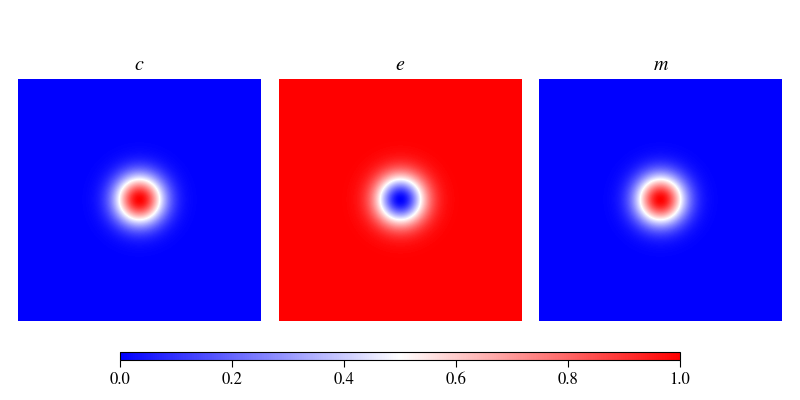
\includegraphics[width=\textwidth]{resources/images/2D_initial_conditions_homogenous_ECM.png}
    \caption{Visualization of the initial value distribution for an experiment in two space dimensions with a homogenous extracellular matrix}
    \label{fig:2D_homogenous_ECM_initial}
\end{figure}
Figure~\ref{fig:2D_homogenous_ECM_initial} shows a 2D plot of the initial conditions using the homogenous extracellular matrix structure. For all three images you see that at the center there is either a high concentration, tumor cell density and matrix degrading enzymes concentration or a low concentration, the extracellular matrix.

\begin{longtable}{|c c c c c c c c c c|}
    \hline
    Figure & Linestyle & $d_c$ & $\gamma$ & $\mu_1$ & $\eta$ & $\mu_2$ & $d_m$ & $\alpha$ & $\beta$ \\ [0.5ex] 
    \hline\hline
    \endfirsthead
    \hline
    Figure & Linestyle & $d_c$ & $\gamma$ & $\mu_1$ & $\eta$ & $\mu_2$ & $d_m$ & $\alpha$ & $\beta$ \\ [0.5ex] 
    \hline\hline
    \endhead
    \hline \multicolumn{10}{|r|}{{continued on next page}} \\ \hline
    \endfoot
    \endlastfoot
    \ref{fig:unadjsuted_replication} & \sampleline{} & $1\cdot 10^{-3}$ & $0.005$ & $0$ & $10$ & $0$ & $1\cdot 10^{-3}$ & $0.1$ & $0$\\  \hline
    \ref{fig:replication_alpha_comparison} & \sampleline{dash pattern=on .7em off .2em on .05em off .2em} & $1\cdot 10^{-3}$ & 0.005 & 0 & 10 & 0 & $1\cdot 10^{-3}$ & 0.2 & 0\\  \hline
    \ref{fig:replication_alpha_comparison} & \sampleline{dotted} & $1\cdot 10^{-3}$ & 0.005 & 0 & 10 & 0 & $1\cdot 10^{-3}$ & 0.3 & 0\\  \hline
    \ref{fig:replication_alpha_comparison} & \sampleline{} & $1\cdot 10^{-3}$ & 0.005 & 0 & 10 & 0 & $1\cdot 10^{-3}$ & 0.35 & 0\\  \hline
    \ref{fig:replication_alpha_comparison} & \sampleline{dashed} & $1\cdot 10^{-3}$ & 0.005 & 0 & 10 & 0 & $1\cdot 10^{-3}$ & 0.4 & 0\\  \hline
    \ref{fig:replication_dc_comparison} & \sampleline{dash pattern=on .7em off .2em on .05em off .2em} & $1\cdot 10^{-3}$ & 0.005 & 0 & 10 & 0 & $1\cdot 10^{-3}$ & 0.3546 & 0\\  \hline
    \ref{fig:replication_dc_comparison} & \sampleline{dotted} & $1\cdot 10^{-4}$ & 0.005 & 0 & 10 & 0 & $1\cdot 10^{-3}$ & 0.3546 & 0\\  \hline
    \ref{fig:replication_dc_comparison} & \sampleline{} & $5\cdot 10^{-4}$ & 0.005 & 0 & 10 & 0 & $1\cdot 10^{-3}$ & 0.3546 & 0\\  \hline
    \ref{fig:replication_dc_comparison} & \sampleline{dashed} & $1\cdot 10^{-5}$ & 0.005 & 0 & 10 & 0 & $1\cdot 10^{-3}$ & 0.3546 & 0\\  \hline
    \ref{fig:replication_gamma_comparison} & \sampleline{dash pattern=on .7em off .2em on .05em off .2em} & $5\cdot 10^{-5}$ & 0.005 & 0 & 10 & 0 & $1\cdot 10^{-3}$ & 0.3546 & 0\\  \hline
    \ref{fig:replication_gamma_comparison} & \sampleline{dotted} & $5\cdot 10^{-4}$ & 0.0055 & 0 & 10 & 0 & $1\cdot 10^{-3}$ & 0.3546 & 0\\  \hline
    \ref{fig:replication_gamma_comparison} & \sampleline{} & $5\cdot 10^{-4}$ & 0.006 & 0 & 10 & 0 & $1\cdot 10^{-3}$ & 0.3546 & 0\\  \hline
    \ref{fig:replication_gamma_comparison} & \sampleline{dashed} & $5\cdot 10^{-4}$ & 0.007 & 0 & 10 & 0 & $1\cdot 10^{-3}$ & 0.3546 & 0\\  \hline
    \ref{fig:basecase_without_proliferation} & \sampleline{} & $5\cdot 10^{-4}$ & 0.0055 & 0 & 10 & 0 & $1\cdot 10^{-3}$ & 0.3546 & 0\\ \hline
    \ref{fig:dc_variation} & \sampleline{dash pattern=on .7em off .2em on .05em off .2em} & $5\cdot 10^{-5}$ & 0.0055 & 0 & 10 & 0 & $1\cdot 10^{-3}$ & 0.3546 & 0\\ \hline
    \ref{fig:dc_variation} & \sampleline{} & $1\cdot 10^{-4}$ & 0.0055 & 0 & 10 & 0 & $1\cdot 10^{-3}$ & 0.3546 & 0\\ \hline
    \ref{fig:dc_variation} & \sampleline{dotted} & $1\cdot 10^{-3}$ & 0.0055 & 0 & 10 & 0 & $1\cdot 10^{-3}$ & 0.3546 & 0\\ \hline
    \ref{fig:gamma_variation} & \sampleline{dotted} & $5\cdot 10^{-4}$ & 0.002 & 0 & 10 & 0 & $1\cdot 10^{-3}$ & 0.3546 & 0\\ \hline
    \ref{fig:gamma_variation} & \sampleline{} & $5\cdot 10^{-4}$ & 0.008 & 0 & 10 & 0 & $1\cdot 10^{-3}$ & 0.3546 & 0\\ \hline
    \ref{fig:gamma_variation} & \sampleline{dashed} & $5\cdot 10^{-4}$ & 0.01 & 0 & 10 & 0 & $1\cdot 10^{-3}$ & 0.3546 & 0\\ \hline
    \ref{fig:gamma_2D_plot} & \sampleline{} & $5\cdot 10^{-4}$ & 0.1 & 0 & 10 & 0 & $1\cdot 10^{-3}$ & 0.3546 & 0\\ \hline
    \ref{fig:gamma_pol_comparison} & \sampleline{} & $5\cdot 10^{-4}$ & 0.1 & 0 & 10 & 0 & $1\cdot 10^{-3}$ & 0.3546 & 0\\ \hline
    \ref{fig:eta_variation} & \sampleline{dotted} & $5\cdot 10^{-4}$ & 0.0055 & 0 & 2 & 0 & $1\cdot 10^{-3}$ & 0.3546 & 0\\ \hline
    \ref{fig:eta_variation} & \sampleline{} & $5\cdot 10^{-4}$ & 0.0055 & 0 & 12 & 0 & $1\cdot 10^{-3}$ & 0.3546 & 0 \\ \hline
    \ref{fig:eta_variation} & \sampleline{dotted} & $5\cdot 10^{-4}$ & 0.0055 & 0 & 20 & 0 & $1\cdot 10^{-3}$ & 0.3546 & 0 \\ \hline
    \ref{fig:dm_variation} & \sampleline{dotted} & $1\cdot 10^{-3}$ & 0.0055 & 0 & 10 & 0 & 0.00001 & 0.3546 & 0 \\ \hline
    \ref{fig:dm_variation} & \sampleline{} & $1\cdot 10^{-4}$ & 0.0055 & 0 & 10 & 0 & 0.001 & 0.3546 & 0 \\ \hline
    \ref{fig:dm_variation} & \sampleline{dashed} & $1\cdot 10^{-5}$ & 0.0055 & 0 & 10 & 0 & 0.1 & 0.3546 & 0 \\ \hline
    \ref{fig:alpha_variation} & \sampleline{dotted} & $5\cdot 10^{-4}$ & 0.0055 & 0 & 10 & 0 & $1\cdot 10^{-3}$ & 0 & 0 \\ \hline
    \ref{fig:alpha_variation} & \sampleline{} & $5\cdot 10^{-4}$ & 0.0055 & 0 & 10 & 0 & $1\cdot 10^{-3}$ & 0.6 & 0 \\ \hline
    \ref{fig:alpha_variation} & \sampleline{dotted} & $5\cdot 10^{-4}$ & 0.0055 & 0 & 10 & 0 & $1\cdot 10^{-3}$ & 1.0 & 0 \\ \hline
    \ref{fig:beta_variation} & \sampleline{dotted} & $5\cdot 10^{-4}$ & 0.0055 & 0 & 10 & 0 & $1\cdot 10^{-3}$ & 0.3546 & 0.1 \\ \hline
    \ref{fig:beta_variation} & \sampleline{} & $5\cdot 10^{-4}$ & 0.0055 & 0 & 10 & 0 & $1\cdot 10^{-3}$ & 0.3546 & 0.01 \\ \hline
    \ref{fig:beta_variation} & \sampleline{dotted} & $5\cdot 10^{-4}$ & 0.0055 & 0 & 10 & 0 & $1\cdot 10^{-3}$ & 0.3546 & 0.005 \\ \hline
    \ref{fig:dc_gamma_variation} - left& \sampleline{dotted} & $5\cdot 10^{-5}$ & 0.001 & 0 & 10 & 0  & $1\cdot 10^{-3}$ & 0.3546 & 0 \\ \hline
    \ref{fig:dc_gamma_variation} - left & \sampleline{} & $5\cdot 10^{-5}$ & 0.01 & 0 & 10 & 0 & $1\cdot 10^{-3}$ & 0.3546 & 0 \\ \hline
    \ref{fig:dc_gamma_variation} -right & \sampleline{dotted} & $1\cdot 10^{-3}$ & 0.001 & 0 & 10 & 0 & $1\cdot 10^{-3}$ & 0.3546 & 0 \\ \hline
    \ref{fig:dc_gamma_variation} -right & \sampleline{} & $1\cdot 10^{-3}$ & 0.01 & 0 & 10 & 0 & $1\cdot 10^{-3}$ & 0.3546 & 0 \\ \hline
    \ref{fig:dm_eta_variation} - left & \sampleline{dotted} & $5\cdot 10^{-4}$ & 0.0055 & 0 & 2 & 0 & $1\cdot 10^{-5}$ & 0.3546 & 0 \\ \hline
    \ref{fig:dm_eta_variation} - left & \sampleline{} & $5\cdot 10^{-4}$ & 0.0055 & 0 & 20 & 0 & $1\cdot 10^{-5}$ & 0.3546 & 0 \\ \hline
    \ref{fig:dm_eta_variation} -right & \sampleline{dotted} & $5\cdot 10^{-4}$ & 0.0055 & 0 & 2 & 0 & $1\cdot 10^{-3}$ & 0.3546 & 0 \\ \hline
    \ref{fig:dm_eta_variation} -right & \sampleline{} & $5\cdot 10^{-4}$ & 0.0055 & 0 & 20 & 0 & $1\cdot 10^{-3}$ & 0.3546 & 0 \\ \hline
    \ref{fig:alpha_beta_variation} - left & \sampleline{dotted} & $5\cdot 10^{-4}$ & 0.0055 & 0 & 10 & 0 & $1\cdot 10^{-3}$ & 0.1 & 0.005 \\ \hline
    \ref{fig:alpha_beta_variation} - left & \sampleline{} & $5\cdot 10^{-4}$ & 0.0055 & 0 & 10 & 0 & $1\cdot 10^{-3}$ & 0.1 & 0.1 \\ \hline
    \ref{fig:alpha_beta_variation} -right & \sampleline{dotted} & $5\cdot 10^{-4}$ & 0.0055 & 0 & 10 & 0 & $1\cdot 10^{-3}$ & 1.0 & 0.005 \\ \hline
    \ref{fig:alpha_beta_variation} -right & \sampleline{} & $5\cdot 10^{-4}$ & 0.0055 & 0 & 10 & 0 & $1\cdot 10^{-3}$ & 1.0 & 0.1 \\ \hline
    \ref{fig:dm_alpha_beta_variation_1} - left & \sampleline{dotted} & $5\cdot 10^{-4}$ & 0.0055 & 0 & 10 & 0 & $1\cdot 10^{-5}$ & 0.1 & 0.005 \\ \hline
    \ref{fig:dm_alpha_beta_variation_1} - left & \sampleline{} & $5\cdot 10^{-4}$ & 0.0055 & 0 & 10 & 0 & $1\cdot 10^{-5}$ & 0.1 & 0.1 \\ \hline
    \ref{fig:dm_alpha_beta_variation_1} -right & \sampleline{dotted} & $5\cdot 10^{-4}$ & 0.0055 & 0 & 10 & 0 & $1\cdot 10^{-5}$ & 1.0 & 0.005 \\ \hline
    \ref{fig:dm_alpha_beta_variation_1} -right & \sampleline{} & $5\cdot 10^{-4}$ & 0.0055 & 0 & 10 & 0 & $1\cdot 10^{-5}$ & 1.0 & 0.1 \\ \hline
    \ref{fig:dm_alpha_beta_variation_2} - left & \sampleline{dotted} & $5\cdot 10^{-4}$ & 0.0055 & 0 & 10 & 0 & $1\cdot 10^{-3}$ & 0.1 & 0.005 \\ \hline
    \ref{fig:dm_alpha_beta_variation_2} - left & \sampleline{} & $5\cdot 10^{-4}$ & 0.0055 & 0 & 10 & 0 & $1\cdot 10^{-3}$ & 0.1 & 0.1 \\ \hline
    \ref{fig:dm_alpha_beta_variation_2} -right & \sampleline{dotted} & $5\cdot 10^{-4}$ & 0.0055 & 0 & 10 & 0 & $1\cdot 10^{-3}$ & 1.0 & 0.005 \\ \hline
    \ref{fig:dm_alpha_beta_variation_2} -right & \sampleline{} & $5\cdot 10^{-4}$ & 0.0055 & 0 & 10 & 0 & $1\cdot 10^{-3}$ & 1.0 & 0.1 \\ \hline
    \caption{Overview of all experiments conducted for the model without proliferation and renewal producing 2D output}
    \label{table:2D_experiments_without_proliferation}
\end{longtable}
Table~\ref{table:2D_experiments_without_proliferation} gives a detailed overview of all the experiments done in this section and the parameters used to produce the results. We are considering the model without proliferation of the tumor cells or renewal of the extracellular matrix, therefore both parameters $\mu_1$ and $\mu_2$ are set to zero. In most figures there will be more than one experiment described, the linestyle in table~\ref{table:2D_experiments_without_proliferation} determines which experiment exactly is described by the set of parameters.
    
\subsubsection{Basecase Analysis}
We will start with replicating the first experiment from  Anderson et al.\cite{anderson_mathematical_2000}.  Figure~\ref{fig:anderson_experiment} shows a screenshot of this experiment, unfortunately in low resolution, since the original paper had not included any digital data containing the diagrams of their results.
\begin{figure}[ht!]
    \centering
    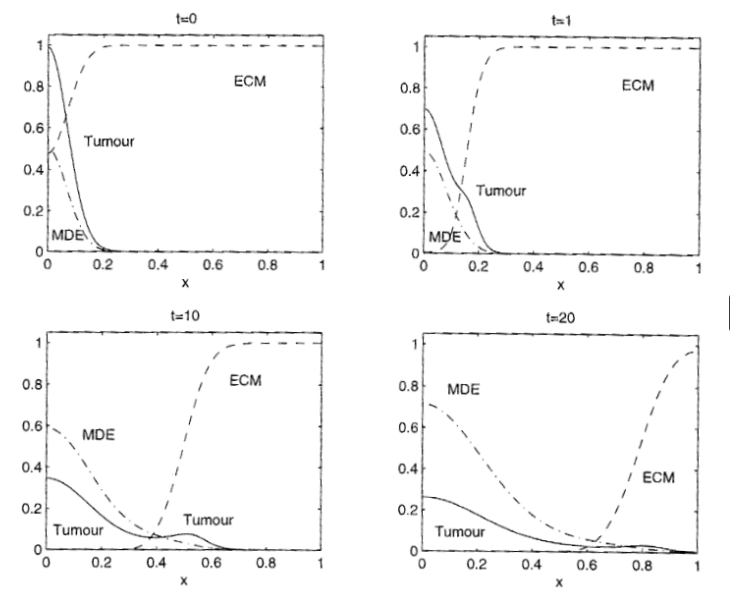
\includegraphics[width=\textwidth]{resources/images/anderson_experiment.png}
    \caption{Andersons first one dimensional experiment using the parameter values $d_c = 1\cdot 10^{-3}, d_m = 1\cdot 10^{-3}, \gamma = 0.005, \eta = 10, \alpha = 0.1, \beta = 0, \mu_1 = 0, \mu_2 = 0$}
    \label{fig:anderson_experiment}
\end{figure}
In figure~\ref{fig:anderson_experiment} you can see that after $t=1$ in their timescale the tumor cells start to develop a secession at the part invading the tissue. This secession propagates to a pointy peak in the later point in time. The concentration of the matrix-degrading enzymes increases continuously and the concentration of the extracellular matrix decreases continuously. We see that their $x$-axis is streched or rescaled to show an intervale from $0$ to $1$. In our case the interval on the plots has only $x$-values from $0$ to $0.5$.
\begin{figure}[ht!]
    \centering
    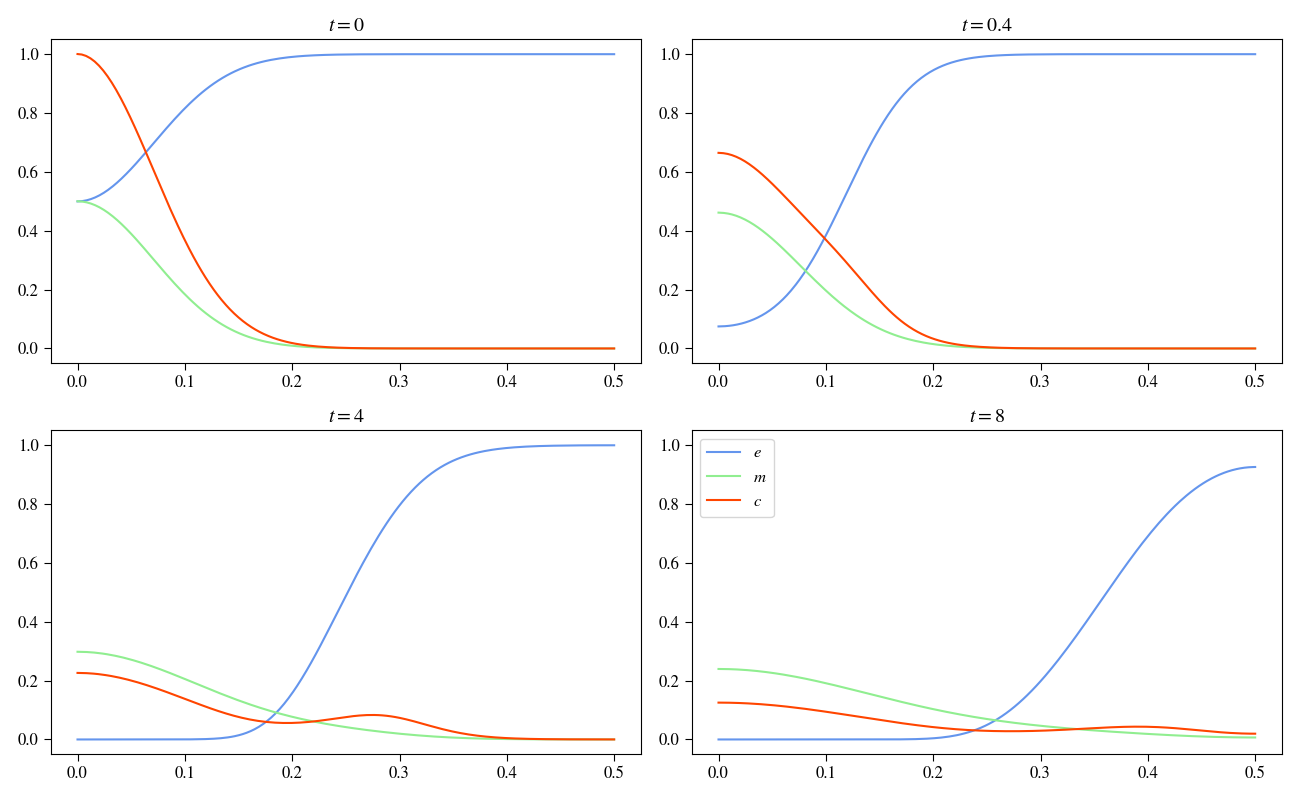
\includegraphics[width=\textwidth]{resources/images/first_replication_POL.png}
    \caption{Results using Anderson et al's parameters produced by applying the Plot Over Line tool}
    \label{fig:unadjsuted_replication}
\end{figure}\
\begin{comment}
\begin{figure}[h!]
    \centering
    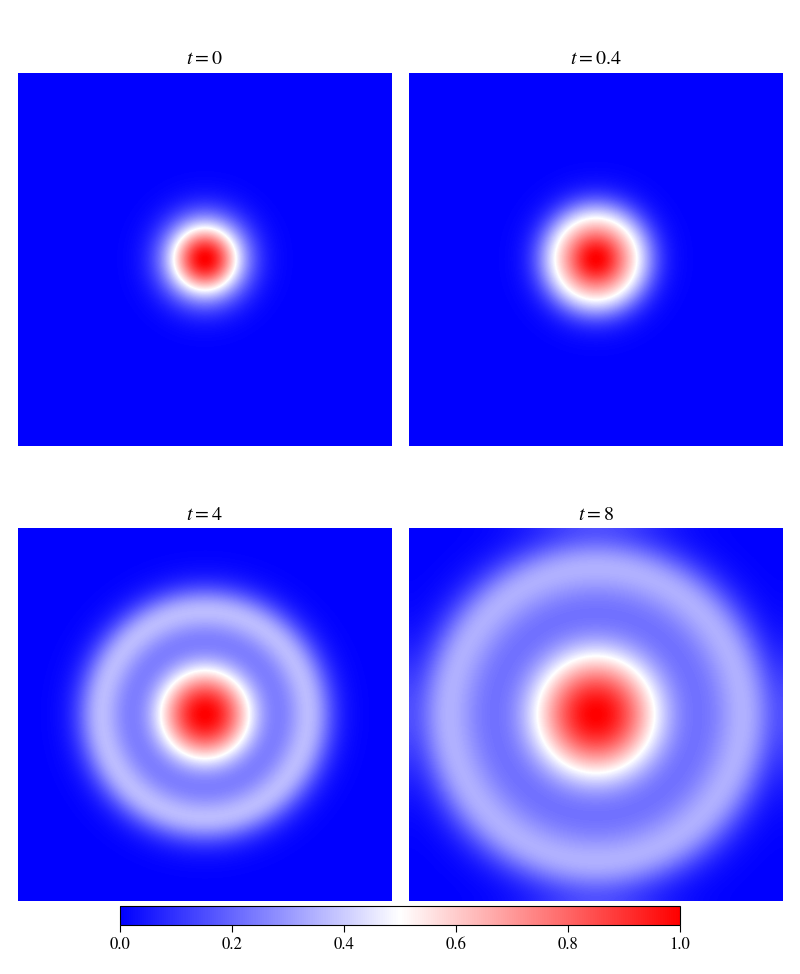
\includegraphics[width=0.5\textwidth]{resources/images/first_replication_2D.png}
    \caption{Results using Anderson et al's parameters 2D tumor cell density plots}
    \label{fig:unadjsuted_replication}
\end{figure}
\end{comment}
Replicating this experiment in two dimensions we start with the same parameters as Anderson et al. had used, $d_c = 1\cdot 10^{-3}, d_m = 1\cdot 10^{-3}, \gamma = 0.005, \eta = 10, \alpha = 0.1, \beta = 0$. Figure~\ref{fig:unadjsuted_replication} shows these results for four different points in time. On the left side you can see the two dimensional plots of the tumor cell density and on the right side you can see plots produced by applying the Plot Over Line tool. As mentioned above we will, for the most part, resort to using only the results produced by the Plot Over Line tool. You can see in the plots of figure~\ref{fig:unadjsuted_replication} on the right side the curves for the three variables are clearly distinguishable and we can estimate their values spacially and temporarily better, than using 2D plots to estimate values.

Starting from the inital values we see that after $t=4$ a very small secession of the tumor cells is starting to form. This secession 
increases in the image at $t=4$, but at $t=8$ it has visibly flattened. This secession is not as pointy as seen in the one dimensional experiments. The interplay of the diffusion and haptotaxis factors determine how big this secession will be that splits from the main lump of the tumor cells and invades the tissue at a faster rate. It will also decide how pointy this secondary lump of tumor cells will be. Biologically this realtion between diffusion and haptotaxis translates to the invasion pace of the tumor cells and the rate of how much of them will remain at the center and how much will invade farther out into the tissue.

Looking at the concentration for the matrix degrading enzymes we see that it is here visily lower than in Anderson et al's experiement. We see little increase across time. This is due to the production factor of $\alpha$. This factor determines how fast the tumor cells produce the matrix-degrading enzymes that are degrading the extracellular matrix and allow the tumor cells to invade the tissue further.

Only the extracellular matrix concentration seems to mimick the behaviour of Anderson et al's experiment. It decreases continuously and in the last image you can see there is still a considerable amount left.

To replicate Anderson et al's results we will start adjusting the mentioned parameters of diffusion coefficient of the tumor cells, haptotatic coeff of the tumor cells and the production rate of the matrix-degrading enzymes. Making the curves fit prefectly will be impossible due to the high degrees of freedom of the system and the change of dimension. Regradless we will replicate as best as possible with a special focus on the values the variables will take at the origin $x=0$.

\begin{figure}[!htb]
    \centering
    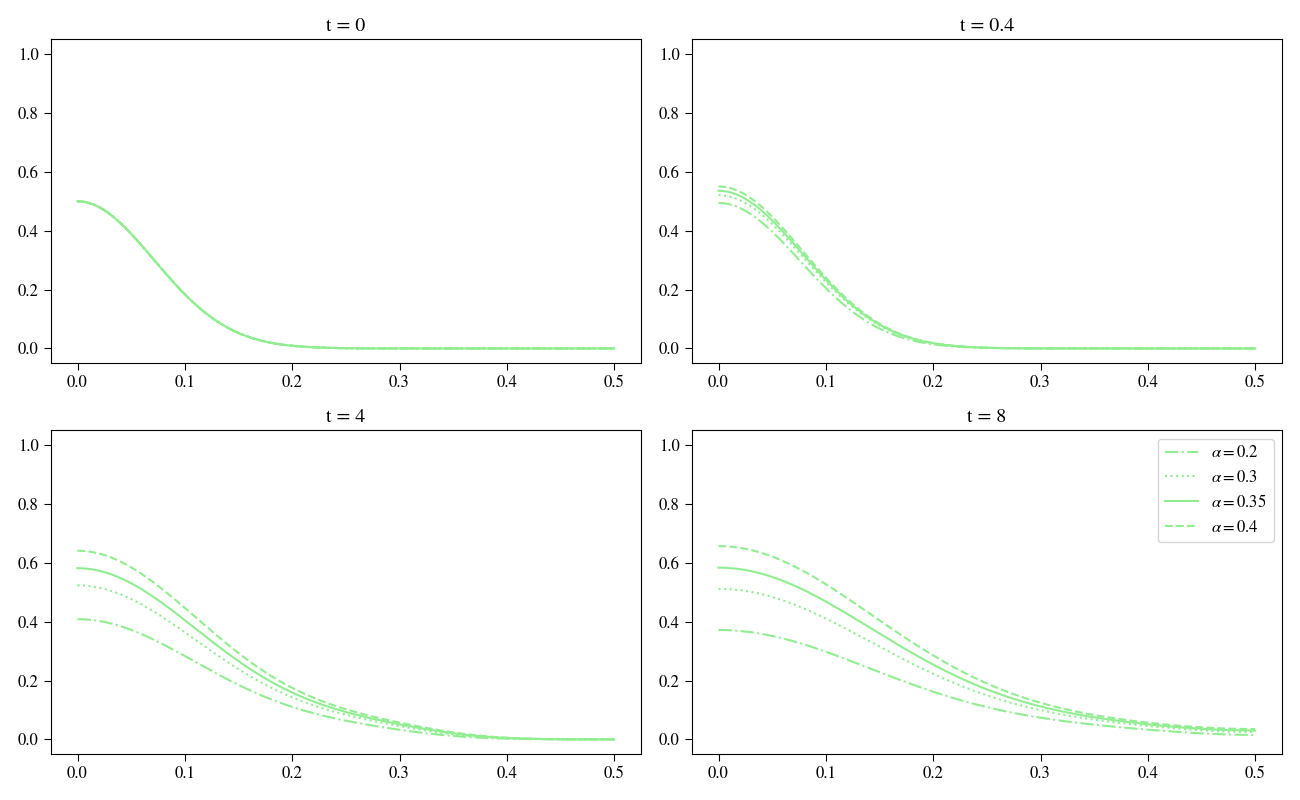
\includegraphics[width=\textwidth]{resources/images/alpha_comparison.png}
    \caption{Comparison of $\alpha$ values to replicate Anderson et al's experiment}
    \label{fig:replication_alpha_comparison}
\end{figure}
Starting with comparing different values for $\alpha$, we see in figuer~\ref{fig:replication_alpha_comparison} a comparison of how this affects the curve for matrix-degrading enzyme concentration. A maximum difference between the compared values of $0.2$ already causes drastic changes as you can see. In Anderson et al's experiment we observe a value of approximately $m(0,1)=0.5$ after, in their timescale, $t=1$ at the origin. This is mimicked best in our case for a value of $\alpha=0.2$. Thoug in the later points in time we see that this value for $\alpha$ is insufficiently low in terms of increase, though choosing $\alpha$ higher than $\alpha=0.4$ results in a accellerated ECM degradation that is too fast. Taking a value between those two allowed our simulations to exhibit the observed behaviour. We choose a value of $\alpha=0.35645$ to use in the later experiments as a basecase.

\begin{figure}[!htb]
    \centering
    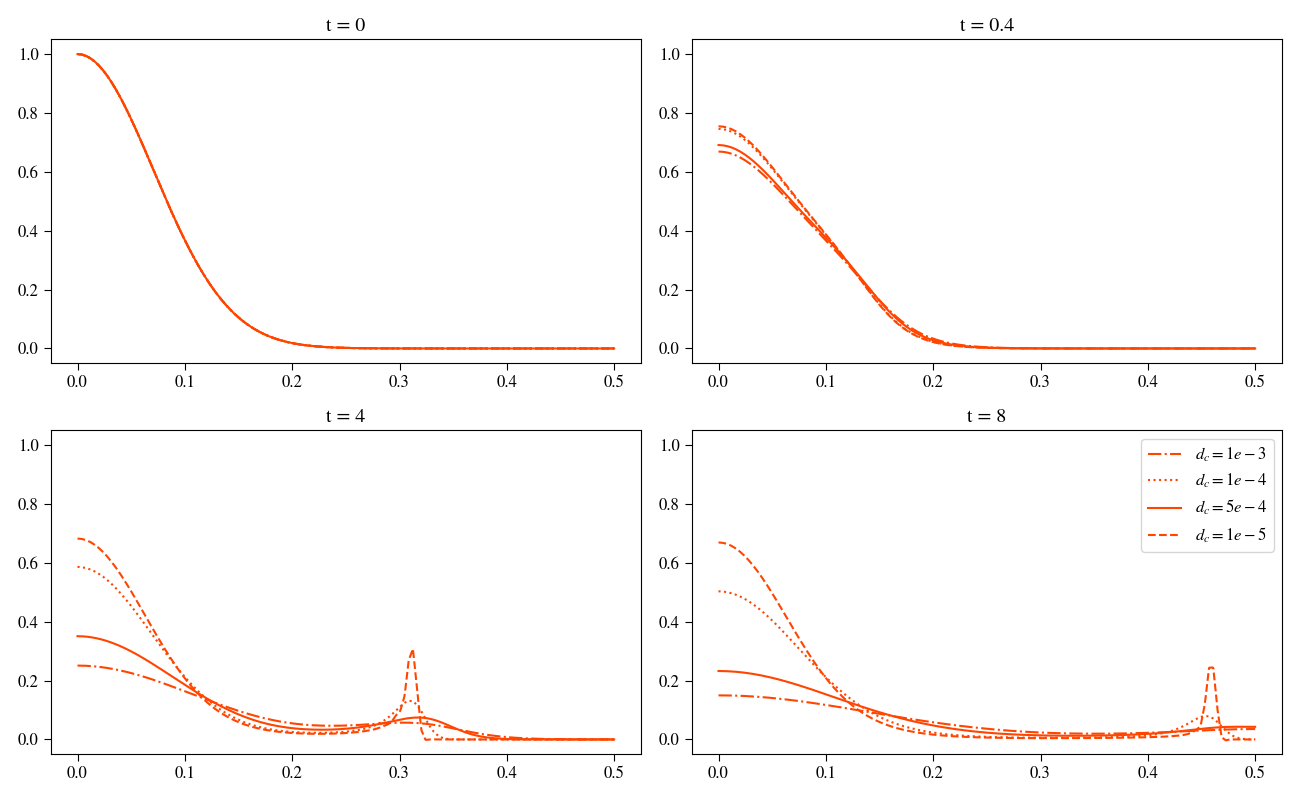
\includegraphics[width=\textwidth]{resources/images/dc_comparison.png}
    \caption{Comparison of $d_c$ values to replicate Anderson et al's experiment}
    \label{fig:replication_dc_comparison}
\end{figure}
Looking now at the diffusion coefficient for the tumor cells, in figure~\ref{fig:replication_dc_comparison} you can see different $d_c$ values compared in regard to the tumor cell concentration. It is clear that with decreasing $d_c$ the sharpness of the secondary lump of cells that forms to invade the tissue drastically increases due to increased effects of haptotaxis being now the main factor to control tumor motility, though we also observe that with decreasing $d_c$ the remaining lump of tumor cells at the origin also increases, due to little diffusion here. Over time we found that $dc=5 \cdot 10^{-4}$ describes Anderson et al's experimental results best for our simulations, with roughly matching density of tumor cells that remains at the origin at all times and, for our case, balanced effects of haptotaxis and diffusion.

\begin{figure}[!htb]
    \centering
    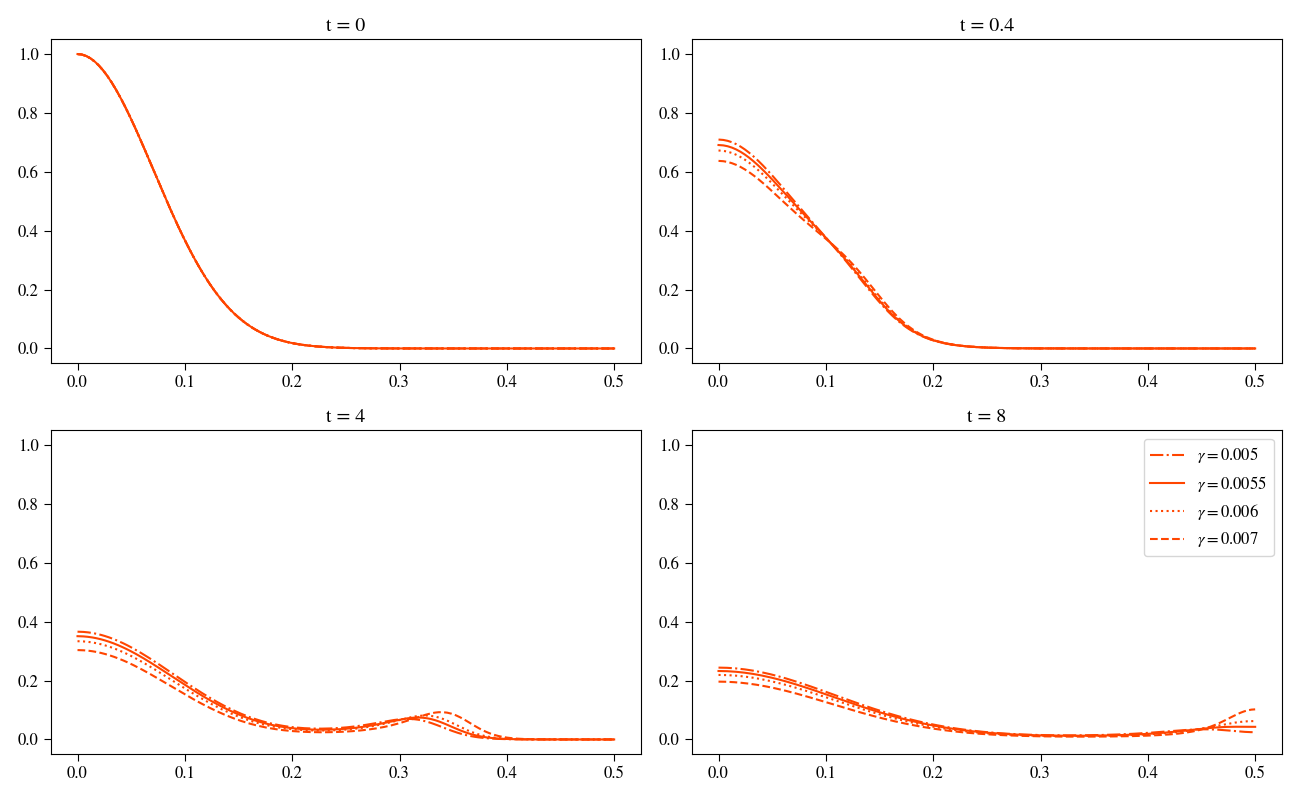
\includegraphics[width=\textwidth]{resources/images/gamma_comparison.png}
    \caption{Comparison of $\gamma$ values to replicate Anderson et al's experiment}
    \label{fig:replication_gamma_comparison}
\end{figure}
At last we want to adjust the haptotatic pull slightly, for this we are looking at a comparision of different $\gamma$ values in figure~\ref{fig:replication_gamma_comparison} depicting the tumor cell density. Comparing our results with Anderson et al's we want a larger secondary lump that invades the tumor cells faster than the one remaining at the origin. For this we need to increase $\gamma$ to increase the haptotaic pull that controls tumor cells motility. In the figure you see that incresing $\gamma$ yields these effects, but increasing it too much results in a too fast invasion pace of the surrounding tissue. Increasing $\gamma$ slightly to $\gamma=0.0055$ is already sufficient to produce the desried effects.

\begin{figure}[h]
    \centering
    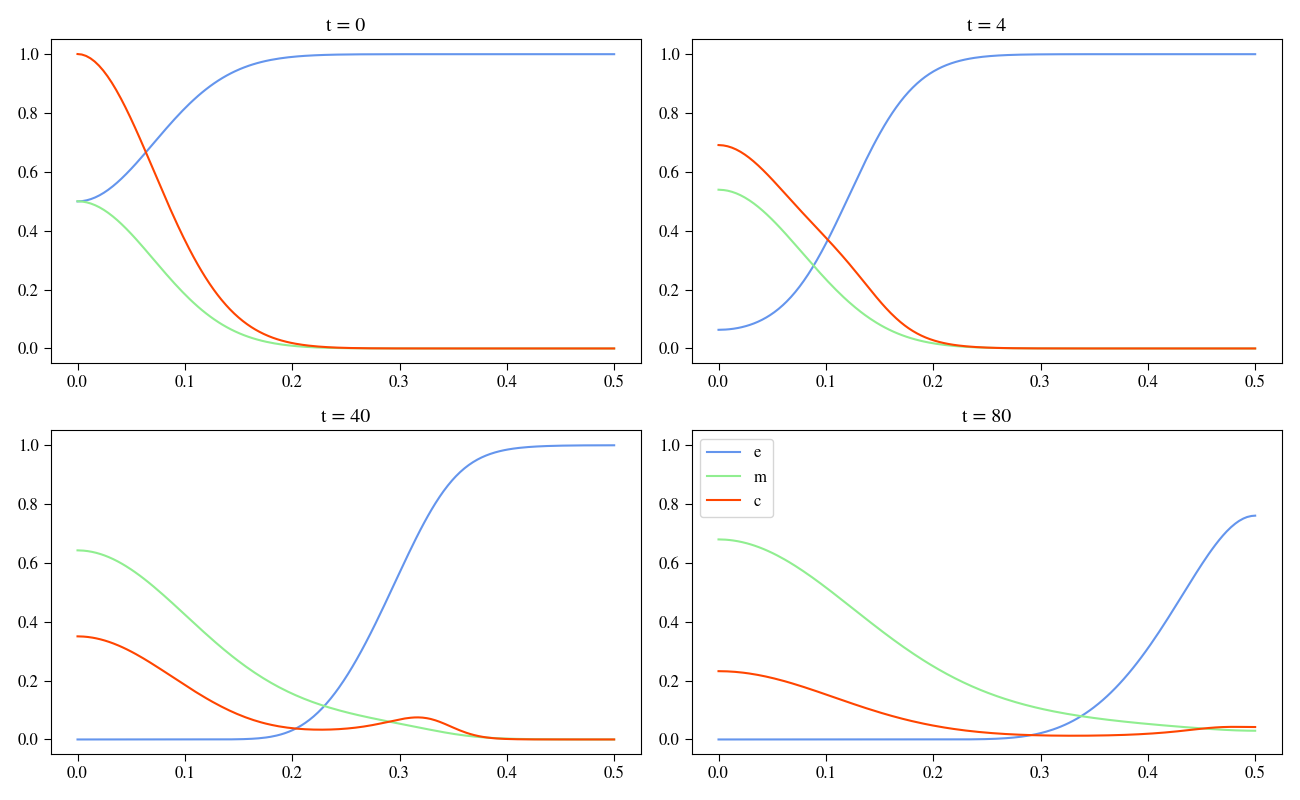
\includegraphics[width=\textwidth]{resources/images/basecase_without_proliferation_.png}
    \caption{Results of using the parameters as described, this experiment will be used as the basecase to compare further experiments to ragarding the model without proliferation and renewal}
    \label{fig:basecase_without_proliferation}
\end{figure}
These adjustments leave us with the final configuration for replicating the system with the curves in figure~\ref{fig:basecase_without_proliferation} and the parameter settings of: $d_c=5\cdot 10^{-4}, \gamma=0.0055, \eta=10, d_m=1\cdot 10^{-3}, \alpha=0.35645, \beta=0$. Comparing our final version with the original experiment we are trying to replicate, figure~\ref{fig:anderson_experiment}, we see the important effects met. We see that the production of the matrix-degrading enzymes fits the original experiment and the motility of the tumor cells also match, with balanced effects of haptotaxis and diffusion.


\subsubsection{Parameter Analysis}
Before we start with the parameter analysis, we will discuss the mathematical intuition concerning the system partial differential equations, equations~\ref{eq:6} to~\ref{eq:10}. 

The equation governing the tumor cell density incorporates in this version only two coefficients regarding its motility, diffusion and haptotaxis. As mentioned during replicating Anderson et al's experiment, the relation between those two factors determines if a secondary lump of tumor cells seccesses itself from the main lump and invades the tissue at a faster rate than the remaining cells, but also how large this lump will be. We saw this behaviour in figure~\ref{fig:replication_dc_comparison}, varying $d_c$ whilst keeping $\gamma$ constant. Diffusive motility depends on the laplacian of the tumor cells themselves, $\Delta c = \frac{\partial c}{\partial x} + \frac{\partial c}{\partial y} + \frac{\partial c}{\partial z}$, which is a fundamental tool in sciences of all sorts to describe the effects of spacial rate of change of a scalar field quantity, in our case tumor cell density, at a specific point in space. Typically this operator has high values where the respective quantity changes rapidly. For the haptotaxis we have a very similiar term $\nabla \cdot (c\nabla e) = \nabla c \cdot \nabla e + \Delta e$. This means that haptotatic effects are not only strong where the concentration of the extracellular matrix changes rapidly but also where both gradients for tumor cell density and extracellular matrix assimilate in direction, thought these effects can also annihilate each other.

The equation describing the concentration of the extracellular matrix models exponential decay of it with taking the concentration of the matrix-degrading enzymes into account. In spacial and temporal positions where both ECM and MDE concentrations are high, we can expect a fast degradation of the extracellular matrix.

The equation modelling the matrix-degrading enzymes combines motility with production/decay terms. The motility of the MDEs is modelled by the same diffusion as the tumor cells, mimicking their behaviour in this regard. The tumor cells are responsible for producing the MDEs, the production is modelled by natural decay, both production and decay are modelled using exponential approaches.

From the replicated results shown in figures~\ref{fig:basecase_without_proliferation}, we saw that if we vary the parameters one at a time the results can vary strongly. We are first going to have a look at how changing one parameter at a time affects the output of the simulation and after this we consider changing multiple parameters simultaneously in the cross variation section. For varying the parameters we assume the other parameters of the system to be constant and use the baseline experiment as their values.

\subsubsection*{$d_c$ Variation}
This parameter describes the diffusive properties of the tumor cells and as Chaplain et al. assumed in~\cite{STEPHANOU200696}, we are also assuming an even distribution of this parameter with $d_c \sim U[1\cdot 10^{-5}, 1\cdot 10^{-3}]$, though in our experiments we encountered numerical instabilities reducing the parameter furhter than $5 \cdot 10^{-5}$. 

As described the intuition is that decreasing $d_c$ will increase the effects haptotaxis and make $\gamma$ more influential. This means the tumor cells will drift faster outward with a bigger secondary lump, forming a pointier leading edge. On the other hand if we increase $d_c$ the effects of haptotaxis will diminish, the tumor cells will be subject to higher diffusion distributing them more evenly in the tissue, additionally there will be less of a secession that is seperated from the main lump of cells. 
\begin{figure}[h!]
    \centering
    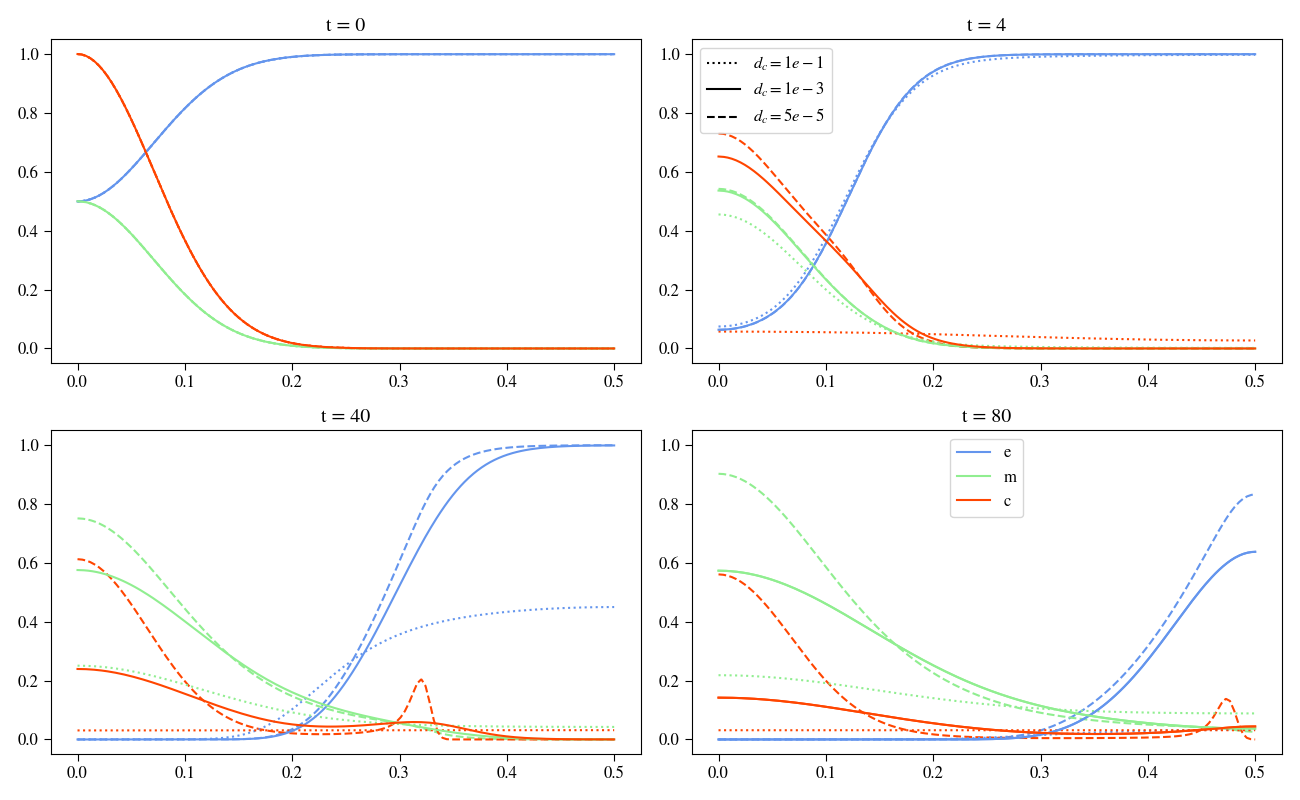
\includegraphics[width=\textwidth]{resources/images/dc_variation.png}
    \caption{Results of varying $d_c$ in the basecase parameter set, keeping the other parameters constant, using the Plot Over Line tool}
    \label{fig:dc_variation}
\end{figure}
Looking at the experiments in figure~\ref{fig:dc_variation}, we can see these assumptions met. The smaller $d_c$ gets the higher the influence of haptotaxis and therefore $\gamma$  will be and vice versa.

Considering the tumor cell denisty curves shown in red, we can after already $t=0.4$ see minor differences. For the two lower values of $d_c$, the solid and dashed curves, we see the tumor cells having a higher concentration at the origin than for the biggest value of $d_c$, dotted curve, nearly overlaying each other. The red dashed curve is considerably lower at the origin though it is stretched  out more than the other two, indicating a faster invasion rate. The other curves describing EDM and MDE concentration don't show any deviations from each other in this point in time.

Looking at the plot results, at time $t=4$, we see the previously observed effects increase. The curves of the tumor cells confirm that with increasing $d_c$ the remaining lump of cells at the origin decreases, distributing the tumor cells more evenly in space and also reducing the effect of haptotaxis, making the secondary lump, that is still visible for the highest diffusion term, less sharp. At this point in time the other two curves also start to show differentiating behaviour. The ECM is degraded faster with increasing $d_c$ and the slope the ECM describes is less steep. Looking at the extracellular matrix we see minor differences in the lower two values for $d_c$. Due to the exponential production of the MDEs by the tumor cells and the more even spread of the tumor cells we see them taking on a lower concentration at the origin, though we can also observe that they have sprach a little bit farther out than the MDE concentrations describing the experiments with lower $d_c$ values.

Studying the last image of $t=8$ we see no new effects, only the already mentioned propagated, with increasing $d_c$ we see a more even spread of the tumor cells and a reduction of the secondary lump leading the invasion of the tissue. For the MDE concentration we observe that there is less concentration in total due to the exponential growth rate, especially at the origin though we also see a more even distribution of them and a slightly faster invasion pace. This causes the extracellular matrix degradation to work faster.

Regarding the sensitiviy of this parameter, it is to say that the higher the value is, the more sensitive the system reacts. Though the lower two values for $d_c$ are only seperated by $5\cdot 10^{-5}$, and we can unfortunately not experiment with $d_c=1 \cdot 10^{-5}$, due to numerical instabilities, the differences between those two were minimal compared to the difference between the higher two values of $d_c$.

From a biological point of view this increase of diffusion might be caused by a change of temperature, electric potential or mechanical pressure differences. The higher diffusion results in more even spread of the two actively moving quantities of tumor cells and matrix-degrading enzymes, degrading their surrounding tissue, the ECM, at a faster rate.

\subsubsection*{$\gamma$ Variation}
$\gamma$ describes the effects of haptotaxis, it is assumed that it is evenly distributed in $\gamma \sim U[0.001,0.01]$, like Anderson et al~\cite{anderson_mathematical_2000} assumed. Like Anderson et al. we are also going to look at values exceeding this region though most likely losing their biological meaning. Inspecting the effects of $\gamma$ we can assume the countering effects on the tumor cells as for varying $d_c$; selecting higher values for $\gamma$ will increase the effects of haptotaxis, creating a larger secondary lump of cells that is being pulled faster into the tissue.
\begin{figure}[h!]
    \centering
    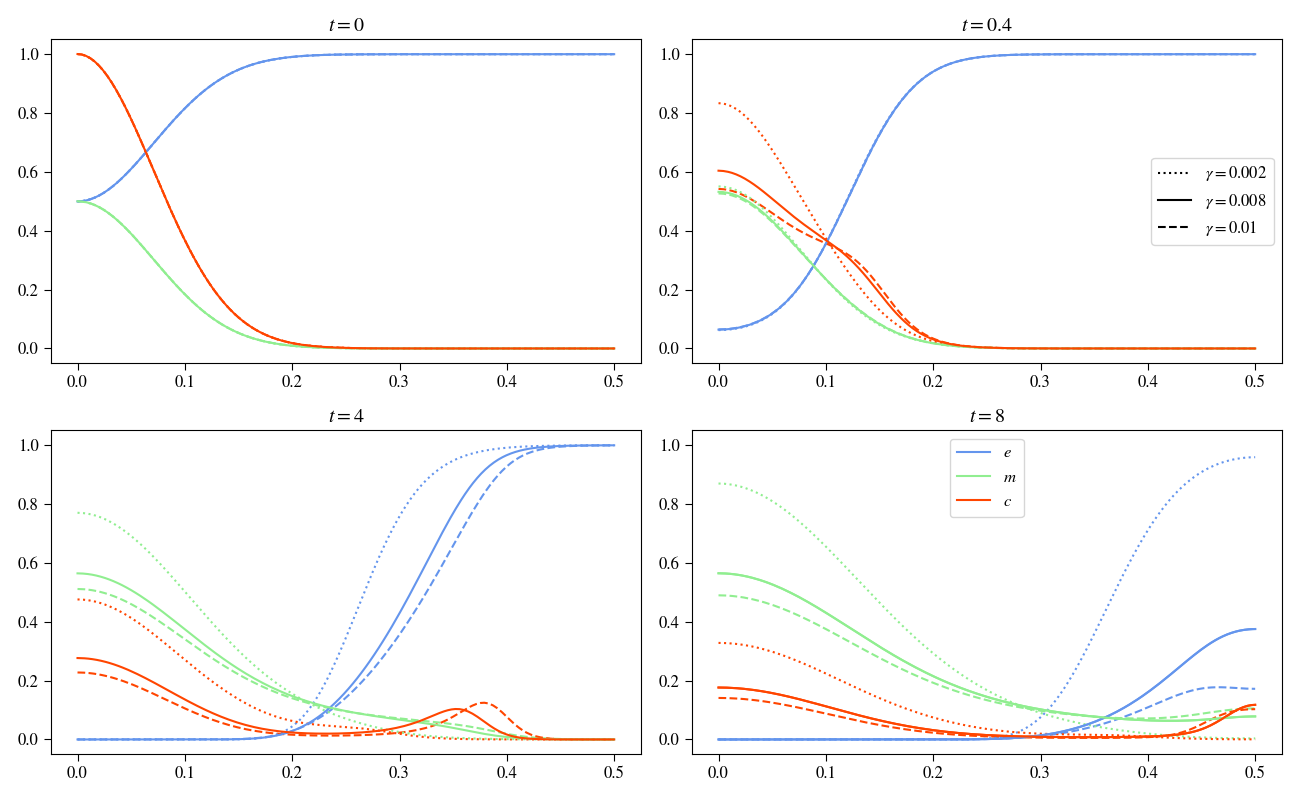
\includegraphics[width=\textwidth]{resources/images/gamma_variation.png}
    \caption{Results of varying $\gamma$ in the basecase parameter set, keeping the other parameters constant, using the Plot Over Line tool}
    \label{fig:gamma_variation}
\end{figure}
The experiments, described in figure~\ref{fig:gamma_variation} verify the expected behaviour.

After $t=0.4$ we already see clear changes for varying $\gamma$, the higher $\gamma$ is set, the more of a secession for the tumor cells is observable, that will later from the secondary lump. The lowest value for $\gamma$, undercutting the one for the basecase, shows no signs of a leading edge forming that invades the tissue seperately. The two higher value for $\gamma$ show little deviation at this point in time. Considering the other two variables extracellular matrix concentration and matrix-degrading enzymes concentration, there is no change visible, still overlaying each other at this temporal point.

The next image shows the simulation after $t=4$ timesteps and here we can clearly see changes in all three variables. 
Whilst the tumor cell density for the values of $0.008$ and $0.01$ differ slightly by the amount of cells that are left at the origin and the distance they have already invaded the surrouding tissue, the curve for the lowest $\gamma$ value, as at $t=0.4$ does not show a secession of the tumor cells that invades the tissue seperately, which causes the tumor cells to stay centered around $x=0$, resulting in a higher denisty of cells there compared to the results of the other experiments. With increasing $\gamma$ the invasion speed also increases, as the dashed line for the tumor cell density shows. For the MDE curve we also observe that the lower $\gamma$ is the more of the concentration is at the origin, which is due to the also higher remaining density of tumor cells at the origin. The ECM concentration shows similiar behaviour as the MDE concentration does, with increasing $\gamma$, the ECM is faster and more evenly degraded, due to the faster invasion of the tissue, the production of matrix-degrading enzymes happens also in regions farther away from the center faster. As we saw varying $d_c$ only little of MDE concentration is needed to efficiently degrade the extracellular matrix, therefore the ECM degradation process happens also faster here.

In the last image at $t=8$ we see the observations from previous points in time confirmed; the higher $\gamma$ the faster the invasion pace of the tumor cells and the more of a secession forms with less tumor cells staying at the origin. The behvviour of the tumor cells causes a higher concentration of MDEs at the origin due to exponential growth and a steeper decline moving outwards. With rising $\gamma$ the ECM is getting degraded faster.

\begin{figure}[h!]
    \centering
    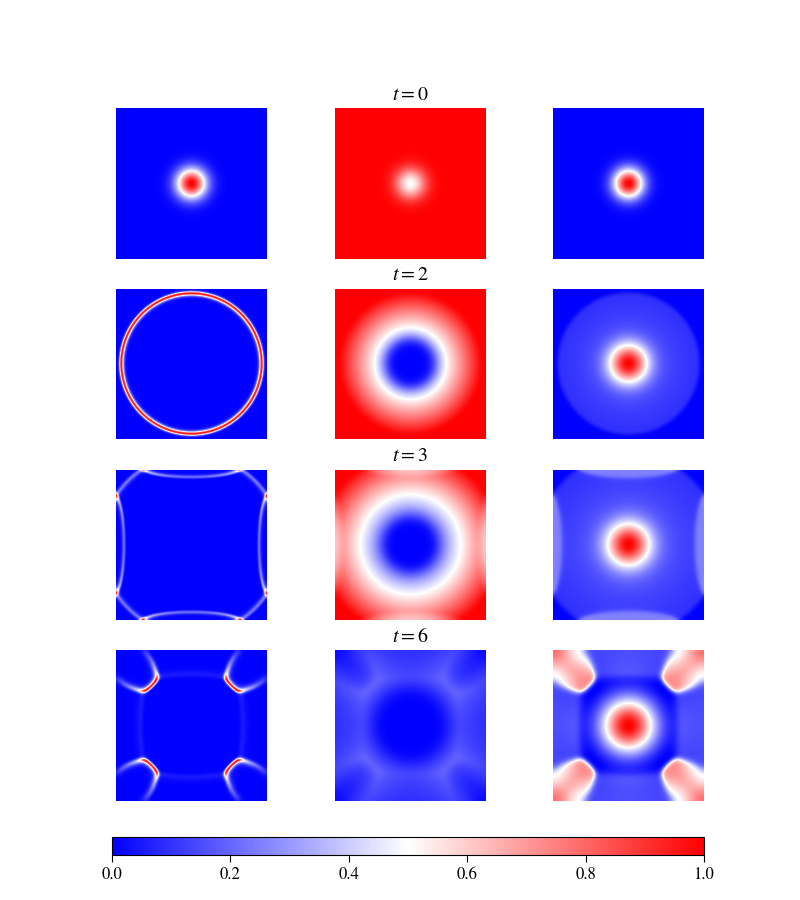
\includegraphics[width=0.85\textwidth]{resources/images/gamma_2D_plot.png}
    \caption{2D plot showing experiment for $\gamma=0.1$, left tumor cell density, right ECM concentration}
    \label{fig:gamma_2D_plot}
\end{figure}
Out of curiousity we are going to take a step further and increase $\gamma$ again by one potence, to $\gamma=0.1$. As previously observed the haptotatic effects pulling the cells into surrounding tissue increase, causing an even faster invasion pace. Yet in this case the invasion pace of the tumor cells is so high there are no cells left at the origin, everything is being pulled into the surrouding tissue. Before finishing the simulation after $t=8$ the tumor cells have reached the border of the doamain $\Omega$. At the border the cells are being reflected, due to the boundry conditions of our model~\ref{eq:9} and~\ref{eq:10}. In figure~\ref{fig:gamma_2D_plot} you can see after $t=2$ the border is reached and at $t=3$ the cells have been reflected to move into the corners, where the ECM concentration is highest. At $t=3$ you can see that the pace of the ECM degradation of the matrix-degrading enzymes has not been able to keep up with the invasion pace of the tumor cells. After being pulled into the corners at $t=3$ and degrading the ECM there, at $t=6$ you see that the tumor cells are being pulled back towards the center of the simulation.

Though this behaviour makes little from a biological perspective, due to the boundry conditions of the system reflecting the movement and the high invasion pace of the tumor cells, it is still interessting to investigate this case, from a numerical perspective.

Though the intuition is met that with increasing $\gamma$ the invasion pace of the tumor cells and matrix-degrading enzymes also rises, we get unexpected behaviour with in the last experiment, there is more of a total ECM concentration left, than in the experiment using $\gamma=0.01$.
Studying those experiments biologically, we know that the term extracellular matrix describes a whole class of different molecules, minearls or proteins, like collagens or enzymes. The different properties of these elements cause varying effects of haptotaxis, for example were the haptotatic effects measured on laminin considerably lower then ones measured on fibronectin, according to Aznavoorian et al.~\cite{article}. In different sites of the human body there will be different constellations of extracellular matrix composition encountered, which will cause the tumor cells, as seen in the numerical experiments to behave differently.

\subsubsection*{$\eta$ Variation}
The parameter $\eta$ controls the degradation process of the extracellular matrix moluecules. Since Anderson et al~\cite{anderson_mathematical_2000} used a value of $\eta=10$ on all their experiments we assumed an even distributed in $\eta \sim U[0, 20]$. The degradation process of the extracellular matrix is modelled using a exponential decay hypothesis so we can expect that increasing $\eta$ also increases the systems sensitivity with respect to the parameter $\eta$. With its role controlling the degradation it will also heavily influence the motility of the tumor cells and therefore also the motility and production rate of the matrix-degrading enzymes. Slower degradation will results in a higher density of tumor cells at the origin which will exponentially produce matrix-degrading enzymes. Though this in turn will increase the ECM degradation. With increasing $\eta$ the ECM is faster degraded and therefore might provoke a faster invasion rate of the tumor cells of the surrounding tissue. The higher $\eta$ is the less MDEs are needed to efficiently degrade the ECM.

\begin{figure}[h!]
    \centering
    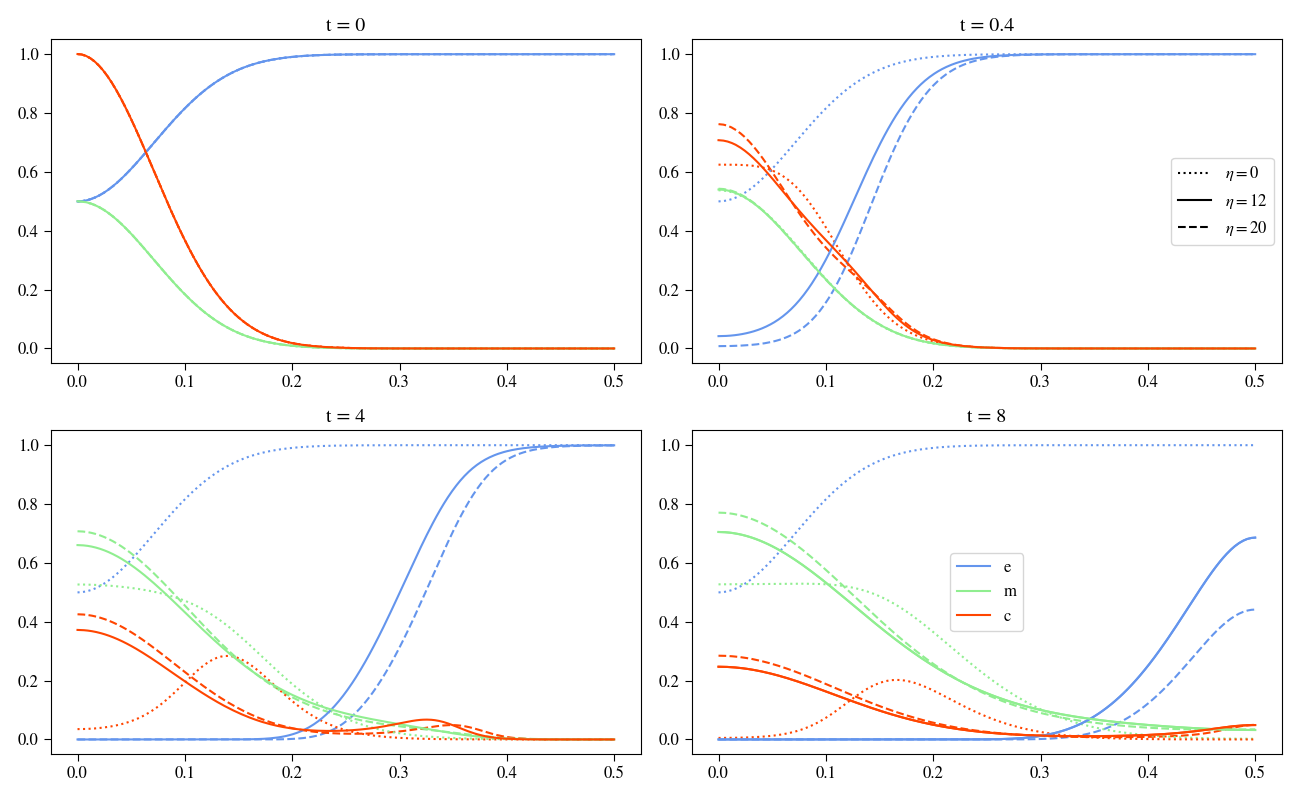
\includegraphics[width=\textwidth]{resources/images/eta_variation.png}
    \caption{Plots show results for varying $\eta$ whilst keeping the other parameters constant, in the images you can see the effects of $\eta=20$ in the dashed curve, $\eta=0$ in the dotted curve and $\eta=12$ in the solid line.}
    \label{fig:eta_variation}
\end{figure}
Inspecting the results in figure~\ref{fig:eta_variation} it is most striking that the slower degradation rate causes a slower tumor invasion. 

For both curves tumor cell density and ECM concentration we see after already $t=4$ big differences. Inspecting the experiment with $\eta=2$ we see that the ECM has only degraded a little, which exposed the tumor cells to stronger haptotatic pull by the ECM in regions closer to zero, comparing it to the other experiments. Though it may look like there is no secondary lump of cells being formed, the contrary is the case, even more cells are being pulled into the tissue, with the ECM slower receeding into the tissue. This smoothes out the bump the other two curves for the tumor cell density show. The same effect is observable comparing the tumor cell density curves for the higher $\eta$ values, with less tumor cells being pulled by the ECM the higher $\eta$ gets. Only the curve for the matrix-degrading enzymes has not been affected by the variation of $\eta$ until now.

The next image at $t=4$ propages the effects on the tumor cells and the ECM. The slower the degradation process happens, the more tumor cells invade into the tissue, and the less of a secession is observable. The movement now also affects the concentration of the matrix-degrading enzymes, with the fewer remaining tumor cells at the origin producing less MDEs, yet we see the distribution of the tumor cells for the lowest case of varying $\eta$ with also a more even distribution of MDEs.

The same goes for the last image, showing the experiments at $t=8$. More even tumor cell and matrix-degrading enzymes distribution across space the slower the ECM is degraded.

As mentioned varying $\gamma$ does the term extracellular matrix include a wide variety of organic or anorganic compounds. The build-up and properties of these compounds therefore vary strongly and motivate this comparison of degradation rate. Some compounds may be degraded faster whilst others are complex needing more time to degrade. 

\subsubsection*{$d_m$ Variation}
$d_m$ describes the diffusion coefficient for the matrix-degrading enzymes. As estimates we use Anderson et al's and Franssen et al's which assume an even distribution of $d_m$ in  $\sim U[1\cdot 10^{-5},1\cdot 10^{-3}]$. Having set $\beta=0$, equation~\ref{eq:8} modelling the temporal development of the matrix-degrading enzymes concentration only depends on c in regard to motility as well as in production. As we saw in experiements before we can expect a high concentration of MDEs in regions where there is a high density of tumor cells and we can expect increased motitlity where the density of the tumor cells rapdily changes. Increasing $d_m$ will cause a faster, more even spread of the MDEs in the surrouding area and therefore the ECM will also be degraded faster.

\begin{figure}[h]
    \centering
    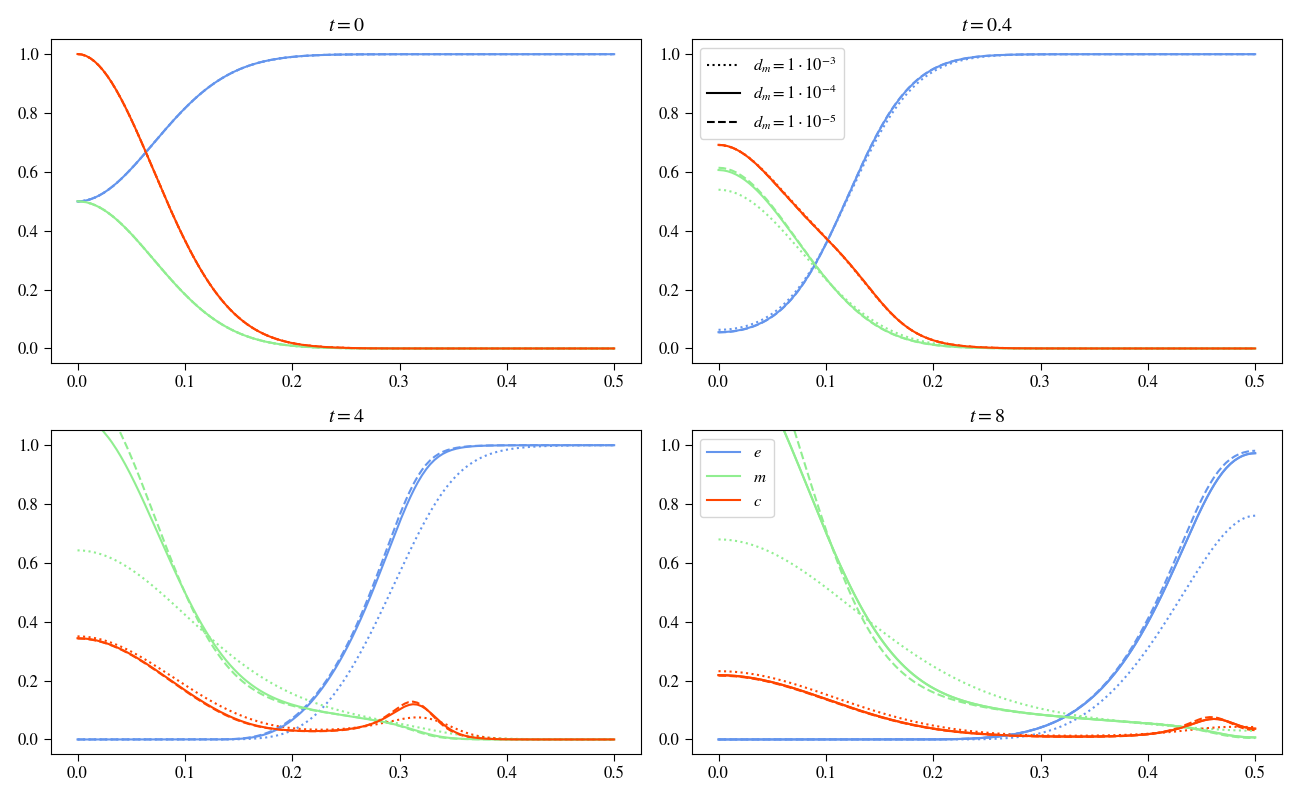
\includegraphics[width=\textwidth]{resources/images/dm_variation.png}
    \caption{Plots show results for varying $d_m$ whilst keeping the other parameters constant, in the images you can see the effects of $d_m=0.1$ in the dashed curve, $d_m=0$ in the dotted curve and $d_m=1\cdot 10^{-3}$ in the solid line.}
    \label{fig:dm_variation}
\end{figure}
Inspecting the results in figure~\ref{fig:dm_variation} we observe that in the second image after $t=0.4$ the curves of the tumor cell density and the ECM are mostly untouched, though looking closely we can see that for the highest $d_m$ value, dotted line, the ECM has at the origin a little higher and farther out a little lower concentration of the ECM. This is caused by the more even distribution of the matrix-degrading enzymes, which reduce the concentration at the origin visibly and invade slightly faster the surrounding tissue at this point in time.

The next image shows the experiments after $t=4$ and we see the differences between lowest $d_m$ value experiment with the other two more pregnantly. The MDE concentration has relative to the other two strongly decreased at the origin, though it has invaded the tissue farther. The ECM has degraded faster and as we saw in the $\eta$ variation, the faster ECM degradation reduces the effects of haptotaxis. The other two experiments differ only visibly in regard to the MDE concentration, though it exceeds the limits of the plot, the concentration at the origin for the lowest diffusive value is considerably higher than for the middle value.

The last image confirms the aforementioned effects, with strongest deviations between the highest $d_m$ experiment with the other two. Again a clearly more even spread of the MDEs with a lower concentration at the origin, a faster ECM degradation and a tumor cell density curves, that, comparing to the other experiments, has less of secession at its leading edge. The two experiments with lower $d_m$ values, still have nearly overlaying tumor cell density and ECM curves, only the MDE concentration differs between the two, showing more even spread for the higher diffusion value, though with a lower value at the origin. 

Seeing those effects we saw our intuition met, though it is to say that looking at the lower two values for $d_m$ the differences here were really modest. Therefore the higher the value for $d_m$ is, the more sensitive the system reacts to this change.

These changes in diffusion, like in the section varying the diffuion coefficient of the tumor cells, might be caused by a multitude of physical influences, temperature, voltage, pressure etc. We see in the results that this change causes a faster degradation of the extracellular matrix molecules but a invasion of the tumor cells that is less aggressive. 
\subsubsection*{$\alpha$ Variation}
\begin{figure}[h]
    \centering
    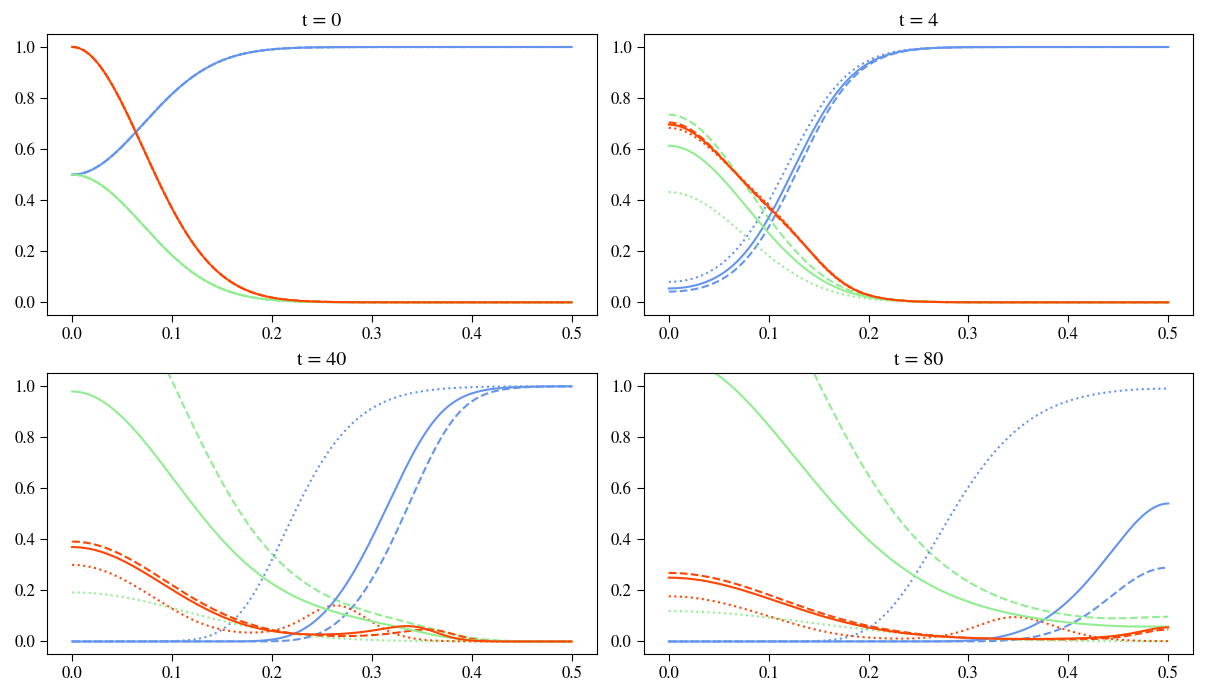
\includegraphics[width=\textwidth]{resources/images/alpha_variation.png}
    \caption{Plots show results for varying $\alpha$ whilst keeping the other parameters constant, in the images you can see the effects of $\alpha=1.0$ in the dashed curve, $\alpha=0$ in the dotted curve and $\alpha=0.6$ in the solid line.}
    \label{fig:alpha_variation}
\end{figure}
The parameter $\alpha$ influences how fast the tumor cells produce matrix-degrading enzymes, we assume it to be evenly distributed with $\alpha \sim U[0, 1.0]$, since in the original paper Anderson et al. assumed the same range. Trying to replicate Anderson et al's experiment we already saw how varying $\alpha$ affects the simulation results. With growing $\alpha$ we will see a higher concentration of MDEs especially in regions where the tumor cell density is high. More MDEs will cause a faster degradation of the ECM first due to having more of them, but also because since more of them are subject to diffusion they will spread faster in the tissue. Faster ECM degrading could mean increased invasion pace of the tumor cells. As we saw in the previous experiments varying $d_c$, the MDE concentration can take on values higher than one, we can also expect this here when $\alpha$ is sufficiently high. 

The second image of figure~\ref{fig:alpha_variation} describes the experiments after $t=0.4$. We can see the differences in the MDE curves for the different values of $\alpha$ clearly. The other curves show also slight deviations, the higher $\alpha$ is, the faster the ECM degradation. Looking closely we can observe for the tumor cell density that the increased rate of ECM degradation results, as previously already seen, in a curve with less of a bump that will later form the secession invading the surrounding tissue, due to smaller haptotatic influences at the origin.

The next point in time at $t=4$, shows the previous mentioned effects in an reinforced way. For $\alpha=0$ the MDEs have no producing factor and the curve flattens due to diffusion, though the extracellular matrix has degraded visibly, yet by a considerably slower rate. This experiment has the lowest denstiy of tumor cells at the origin, though the biggest secondary lump of cells that invades the tissue. This behaviour is due to the longer exposition of strong haptotatic influences near the origin region, which pulls more cells outward to invade.
The solid curves describing $\alpha = 0.6$ show that at this point in time they have almost reached a concentration of one at the center, which will be exceeded at the later time step. The faster ECM concentration compared to the lowest $\alpha$ experiment has also pulled less of the tumor cells outward, though at a faster invasion pace. 
Looking at the highest $\alpha$ experiment, the MDE concentration already exceeds one, the ECM degradation is happening at a faster rate and the invasion of the tumor cells is happening faster, though with a lower density.

In the last timestep we see that the MDE curve of both $\alpha=0.6$ and $\alpha=1.0$ have exceeded one. For the dotted curve of the MDE, we have a good example of diffusion distributing the concentration throughout space, without changing its overall volume. At the border regions we see that the dotted curve is also the only one that has not yet degraded any ECM in this area, whilst the other two experiments show that there is only a little ECM concentration left to degrade. 
The tumor cells confirm the, in the previous timestep mentioned, effects of faster invasion pace with rising $\alpha$ though with at a thinner density.


Our initial assumptions were correct with a faster degradation pace due to higher MDE concentration and therefore a faster invasion pace of the tumor cells. Though it is interesting to see that the smaller $\alpha$, more of the tumor cells are being pulled into the tissue.

Whilst it makes from a numerical perspective sense that the concentration of MDEs can exceed one, it might make sense to introduce a finer grid or adapt the model in other ways, since judging from a continuous perspective it does not really make sense that at a certain point in space there are more than one entities, occupying this space.

Biologically seen the production of matrix-degrading enzymes can have many causes. During many natural processes like tissue repair or remodelling, the extracellular matrix must be degraded, which is controlled by cells producing enzymes that in turn are responsible for producing matrix-degrading enzymes. This control flow can be interrupted by malignant cells stimulating the production of MDEs, without any repair or remodelling tasks to perfrom. Considering no or reduced MDE production we can regard this case as the consequence of a treatment by a drug. On the other hand since there are plenty of different extracellular matrix molecules, they also may have different rates of production.

\subsubsection*{$\beta$ Variation}
The factor $\beta$ controls the decay of the matrix-degrading enzymes and the results of its variation are shown in figure~\ref{fig:beta_variation}. Using Kolev et al's estimate for $\beta$ in \cite{Kolev2010} we started experimenting with $\beta=0.07$. Considering the results we can assume an even distribution of $\beta$ in $\beta \sim U[0.005, 0.1]$. Interestingly $\alpha$ and $\beta$ are, as their respective distribution and also the experiments will confirm, not of the same magnitude. Whilst the MDEs are produced by the tumor cells, their decay is controlled by the MDEs themselves. With this model it is assumed that the tumor cells don't proliferate, which makes their total amount constant. In contrast to this the MDEs are produced by the tumor cells and are expected to change their amount over time due to production or decay. This makes the decay rate of the MDEs more variable, because of the changing amount of total MDEs, causing the change of effective magnitude.

We can assume that with introducing $\beta$ foremost the MDE curve will be lower, influcencing the ECM degrading process and therefore also the invasion pace and the diffusion-haptotatic effects on the tumor cells. 

\begin{figure}[h]
    \centering
    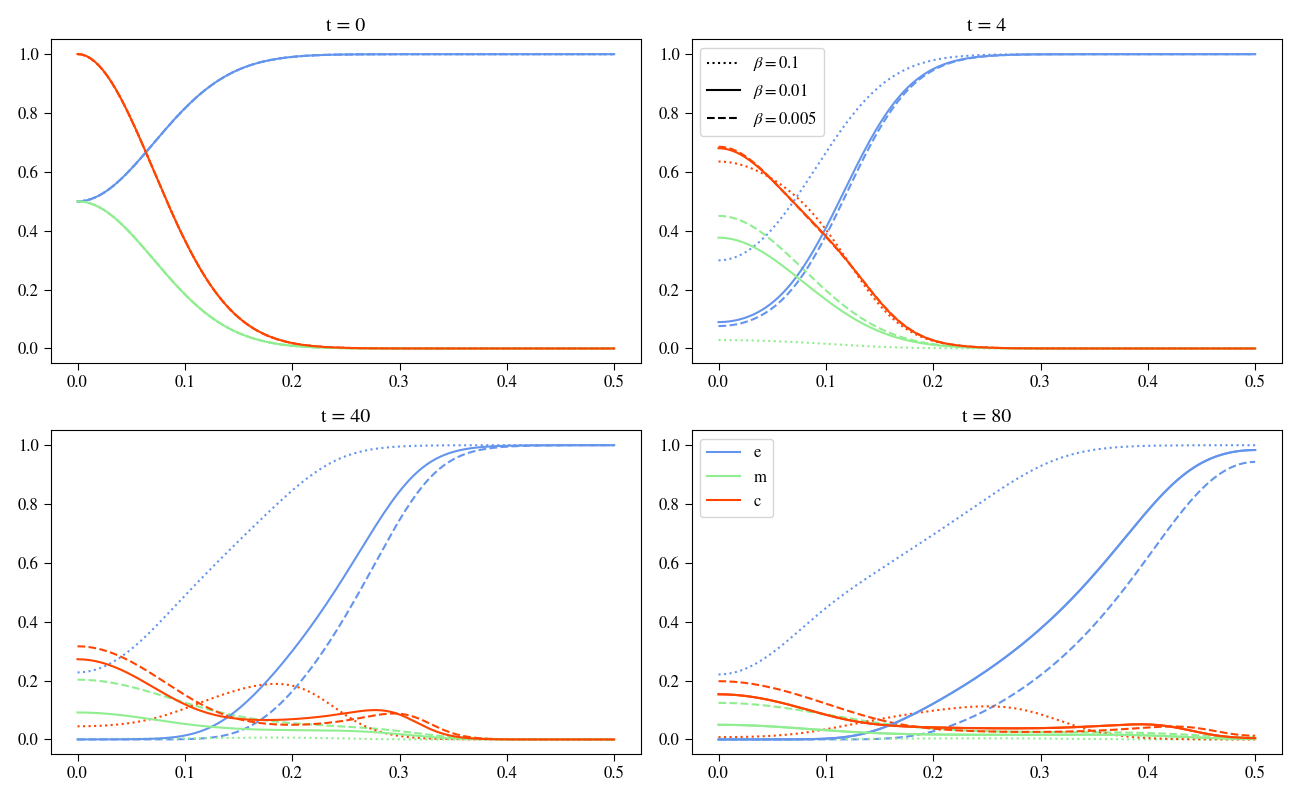
\includegraphics[width=\textwidth]{resources/images/beta_variation.png}
    \caption{Plots show results for varying $\beta$ whilst keeping the other parameters constant, in the images you can see the effects of $\beta=0.005$ in the dashed curve, $\beta=0.1$ in the dotted curve and $\beta=0.01$ in the solid line.}
    \label{fig:beta_variation}
\end{figure}
As we see from the results in figure~\ref{fig:beta_variation} a value of $\beta=0.1$ is sufficient to after already $t=4$ reduce the MDE concentration to nearly zero. This decay rate proves to be too high in our case, outpacing prodcution entirely, with matrix-degrading enzymes concentration vanishing spacially and temporaly completely. The immediate decay of the MDEs causes a drastically slower ECM degradation, yet it has no stopped completely since the tumor cells still produce matrix-degrading enzymes. This slow degradation of extracellular matrix, as we saw previously, creates a haptotatic pull that last at lot longer in regions around the origin, which pulls, in this case, all of the cells outward to invade the tissue, leaving no main lump of tumor cells at the origin. Since more MDEs are produced in regions of high tumor cell density, this causes also a more even degradation of the extracellular matrix, causing a stronger stretch of the tumor cells.

In the other experiments we can observe that with decreasing $\beta$ and slowing down the decay of the matrix-degrading enzymes, first the ECM degradation accellerates and this causes the effects of haptotaxis and diffusion to develop the two lumps of tumor cells, one staying at the center the other invading the tissue, like we saw in all previous experiments.

Since the extracellular matrix can be composed of many different organic and anorganic compounds, the enzymes degrading it are also very diverse. This diversity results in different decay rates, chosing the right one for a specific experiment can be crucial. Whils this variation describes the effects of different enzymes, it can also describe, like for the production of the MDEs, the influence of a drug, to accellerate decay of the matrix-degrading enzymes.

\subsubsection*{Cross Variation}
Having done a variatoin of every parameter of the model,, we saw accellerating effects on the invasion but also countering effects. Now it will be intersting to see how either supporting factors interplay, but also how countering factors affect the simulations, for example how increasing both $\alpha$ and $\beta$, if there can be found some kind of balance. Another interesting experiment will be on how diffusion and haptotaxis behave when increasing or decreasing both factors controlling them.

\subsubsection*{$d_c - \gamma$ Variation}
\begin{figure}[h]
    \centering
    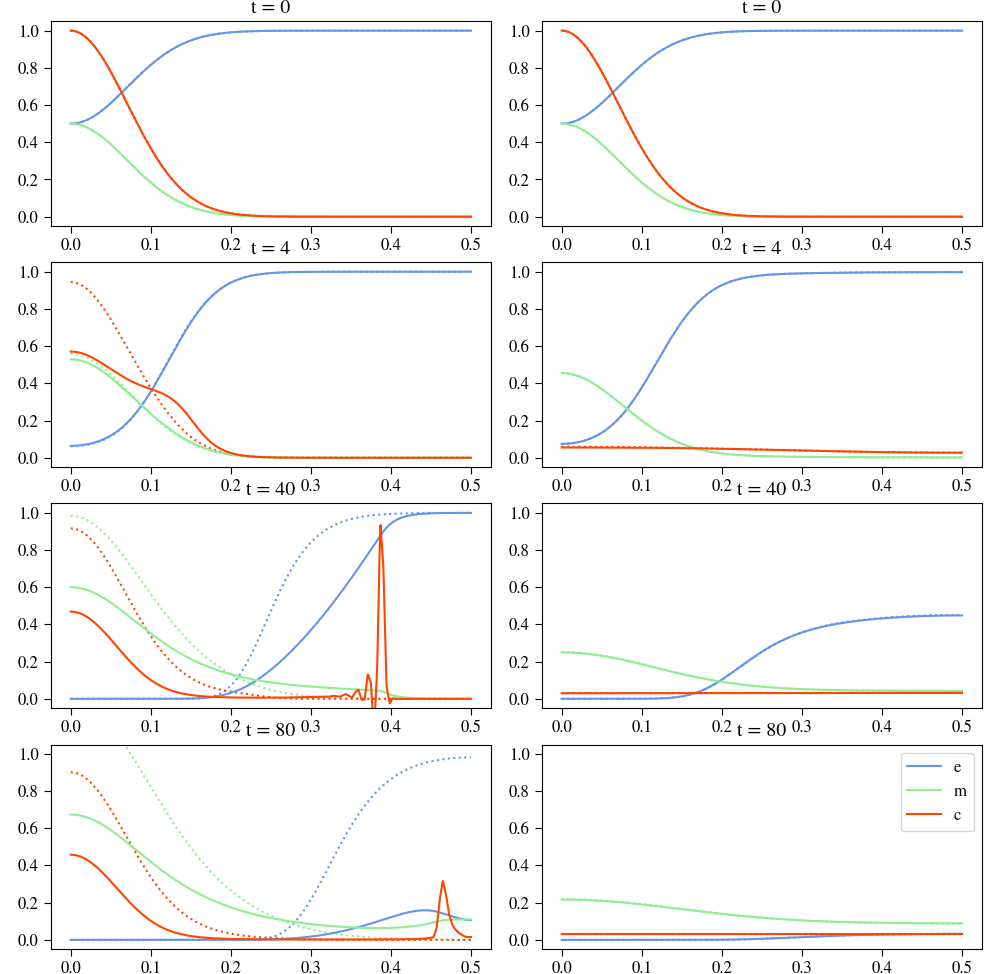
\includegraphics[width=0.85\textwidth]{resources/images/dc_gamma_variation.png}
    \caption{Plots show results for varying both $d_c$ and $\gamma$ whilst keeping the other parameters constant, in the images on the left $d_c$ is set to $d_c=0.00005$ with the solid line showing $\gamma = 0.01$ and the dotted line $\gamma=0.001$ on the right $d_c$ is set to $d_c=0.1$ with the solid line showing $\gamma = 0.01$ and the dotted line $\gamma=0.001$.}
    \label{fig:dc_gamma_variation}
\end{figure}
We therefore started with varying $d_c$ and $\gamma$, and studied for simplicity and overview reasons only the values on their distribution's borders interplaying.

Having set $d_c=0.00005$ and $\gamma=0.001$ we see no secession of the tumor cells, the effects of haptotaxis are too small leaving the tumor cells only subject to diffusion which results in an even distribution process over time, which also causes a slower invasion pace. Because the tumor cells stay in a lump with its maxima at the origin $x=0$ the MDEs also take on their maximum there, moving farther out they also distribute very evenly. This staying with values around the origin of the MDEs causes a slower ECM degradation. Increasing $\gamma=0.01$ we see that the effects of haptotaxis are now pregnantly visible with a very sharp maxima seen at $t=4$, which equals the maxima of the remaining tumor cell lump at $x=0$. Stronger influence of haptotaxis leads to a faster invasion pace of the tumor cells into the tissue and allowing to create matrix-degrading enzymes in their wake, causing a more even distribution compared to $\gamma=0.001$ and also a faster ECM degrading process. 
Looking at the right side of the plot ~\ref{fig:dc_gamma_variation} we see the results for $d_c=0.1$ here for both $\gamma$ values diffusion overshadows the effects of haptotaxis completely, with after already $t=0.4$ having a constant distribution of tumor cells throughout space. Due to this fast spread of tumor cells, the MDEs are also produced evenly throughout space, and an even faster ECM degradataion. 

\subsubsection*{$d_m - \eta$ Variation}
\begin{figure}[h]
    \centering
    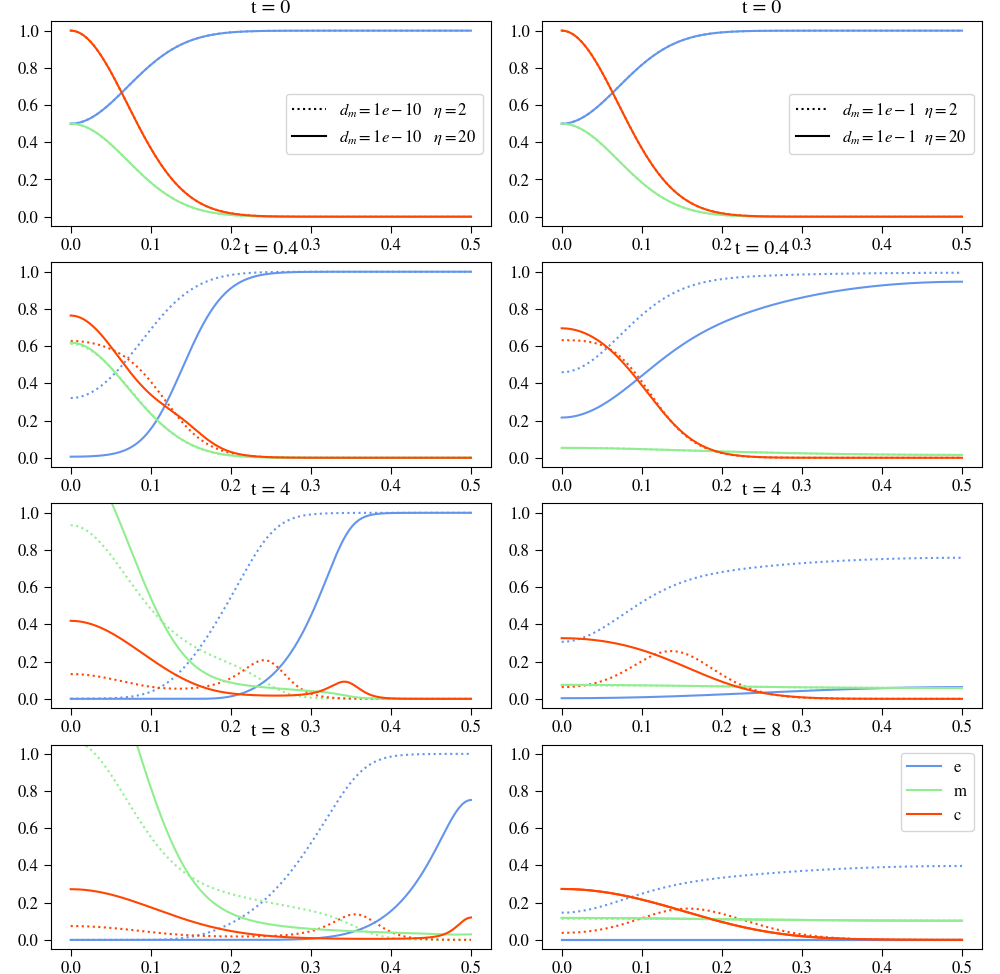
\includegraphics[width=0.85\textwidth]{resources/images/dm_eta_variation.png}
    \caption{Plots show results for varying both $d_m$ and $\eta$ whilst keeping the other parameters constant, in the images on the left $d_m$ is set to $d_m=0.0000000001$ with the solid line showing $\eta = 2$ and the dotted line $\eta=20$ on the right $d_m$ is set to $d_m=0.1$ with the solid line showing $\eta = 2$ and the dotted line $\eta=20$.}
    \label{fig:dm_eta_variation}
\end{figure}

Looking at low values for both $d_m$ and $\eta$ in the figure~\ref{fig:dm_eta_variation}, the dotted curve in the left column, we see that slow diffusion of the matrix-degrading enzymes and slow degradation of the extracellular matrix causes the tumor cells to only develop one lump that invades space, due to stronger haptotatic exposition to a slower degraded ECM, to create larger values for $\nabla (c \nabla e)$, this is also observable for the higher diffusion values and lowwer ECM degrading factors. Having this single lump with a lower maxima and larger length causes the MDEs to produce more evenly farther away from the origin. The low value for the ECM degrading factor results in an overall slower ECM degradation. Looking on the solid line on the left colum we see that increasing $\eta$ enables the tumor cells to develop two hills, one staying at $x=0$ and one invading space by haptotatic pull. Due to a higher density of tumor cells at the origin the MDEs produced there exceed a value of one and ECM degrading happens faster due to first the higher coefficient but also because of a faster invasion pace of matrix-degrading enzymes, due to faster invasion of the tumor cells. Increasing $d_m$ to $d_m=0.1$ causes the MDE concentration to flatten throughout space, taking on a constant distribution in space for one point in time, neglecting the values for $\eta$. Though $\eta$ still has an influence on both tumor cell density and ECM concentration. We see that, as previously mentioned, for $\eta=2$ the degrading happens so slow that the tumor cells form only one lump invading the tissue, with its maxima travelling along the x-axis. In contrast to this for $\eta=20$, we also see only one lump develop though this one stays with it's maxima at the origin. For $\eta=20$ we see that after $t=4$ the ECM has almost completly degraded, making the formation of a secondary lump invading the tissue not possible due to too low haptotatic pull. 

\subsubsection*{$\alpha - \beta$ Variation}
\begin{figure}[h]
    \centering
    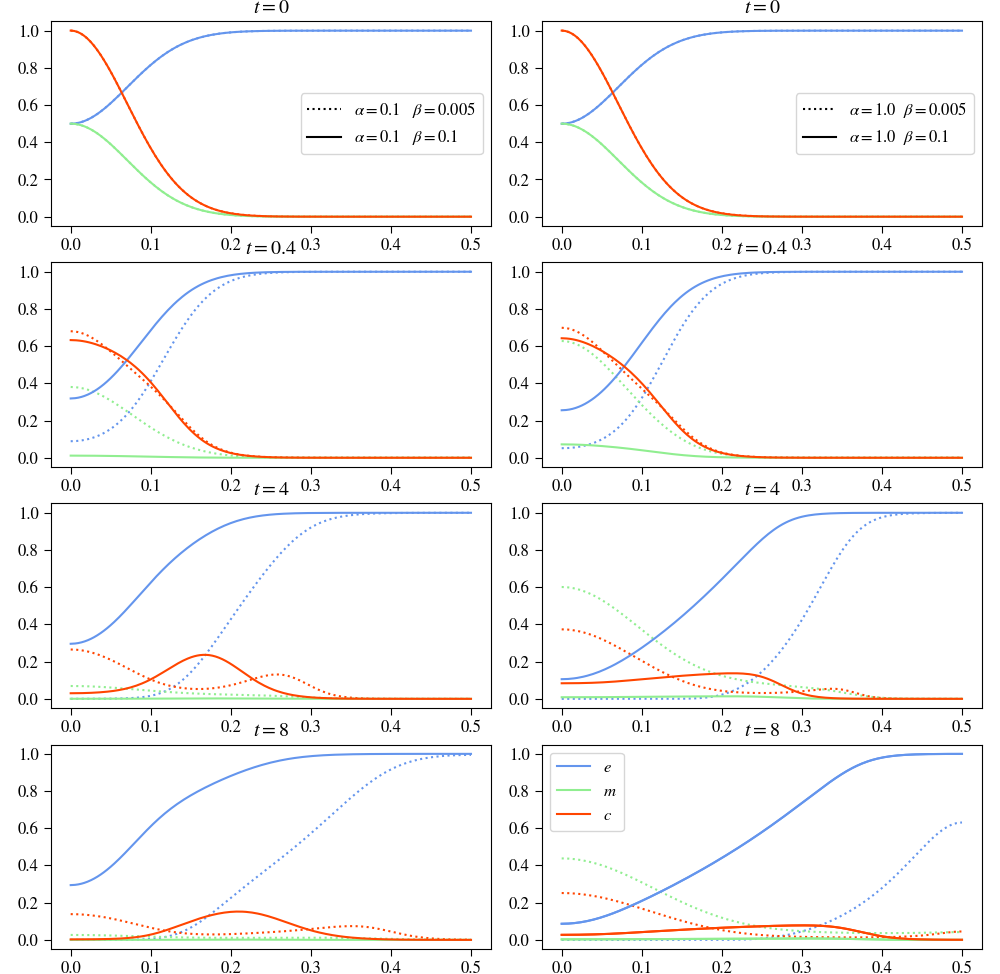
\includegraphics[width=0.85\textwidth]{resources/images/alpha_beta_variation.png}
    \caption{Plots show results for varying both $\alpha$ and $\beta$ whilst keeping the other parameters constant, in the images on the left $\alpha=0.1$ with the solid line showing $\beta = 0.005$ and the dotted line $\beta=0.1$ on the right $\alpha=1.0$ with the solid line showing $\beta = 0.005$ and the dotted line $\beta=0.1$.}
    \label{fig:alpha_beta_variation}
\end{figure}

Looking at figure~\ref{fig:alpha_beta_variation} we see experimental results varying both $\alpha$ and $\beta$. For low MDE production but also low MDE decay we can see that the curve for the MDEs is still visible at up to $t=4$, at $t=8$ it is zero. We see that first the ECM degrading happens faster than for high $\beta$ values and therefore the tumor cells develop two lumps with one invading the tissue the other staying at $x=0$. The maxima for both lumps is lower than in previous experiments, though the cells seem to be more evenly distributed in between the two lumps. Increasing $\beta=0.1$ the MDE curve seems to be zero after already $t=$ and stays there until the end of this experiment. This low concentration of MDEs casuses a slower ECM degrading process and therefore leads the tumor cells to only develop one lump, invading the space, with its maxima moving at the center of this lump. For $\alpha=0.1$ both values for $\beta$ have proven to be to high, decaying the matrix-degrading enzymes too fast to keep up with production.
On the other hand increasing $\alpha$ to $1.0$ and keeping $\beta=0.05$, we see that production outweighs decay, with at the end of the experiment the MDEs still have a concentration of about $0.4$ at $x=0$. For this experiment we seee that the tumor cells develop two lumps indicating that diffusion and haptotaxis effects are also in some balance, and ECM degradation seems to resemble due to similiarities with the basecase for the MDE curve, also the ECM degradation of the basecase experiment.
Increasing both $\alpha$ and $\beta$ we see in the solid line of the right column of figure~\ref{fig:alpha_beta_variation} that decay outweighs production again, after $t=0.4$ we can only see a small remaining portion of matrix-degrading enzymes at the origin. This causes a slower ECM degradataion and therefore to forming only one lump of tumor cells, due to too strong effects of haptotaxis, though this singular lump is streched flat along the x-axis.

\subsubsection*{$d_m - \alpha - \beta$ Variation}
\begin{figure}[h]
    \centering
    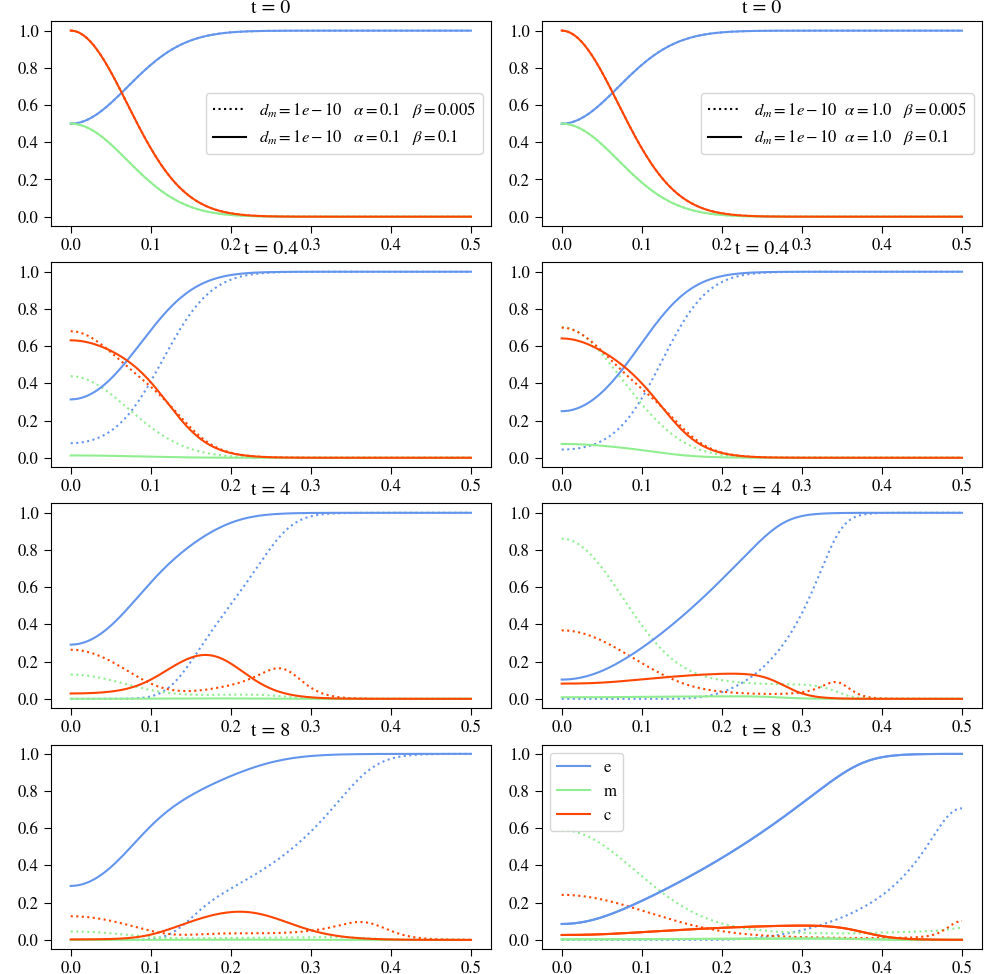
\includegraphics[width=0.85\textwidth]{resources/images/dm_alpha_beta_variation_1.png}
    \caption{Plots show results for varying both $\alpha$ and $\beta$ whilst keeping the other parameters constant, in the images on the left $\alpha=0.1$ with the solid line showing $\beta = 0.005$ and the dotted line $\beta=0.1$ on the right $\alpha=1.0$ with the solid line showing $\beta = 0.005$ and the dotted line $\beta=0.1$.}
    \label{fig:dm_alpha_beta_variation_1}
\end{figure}
\begin{figure}[h]
    \centering
    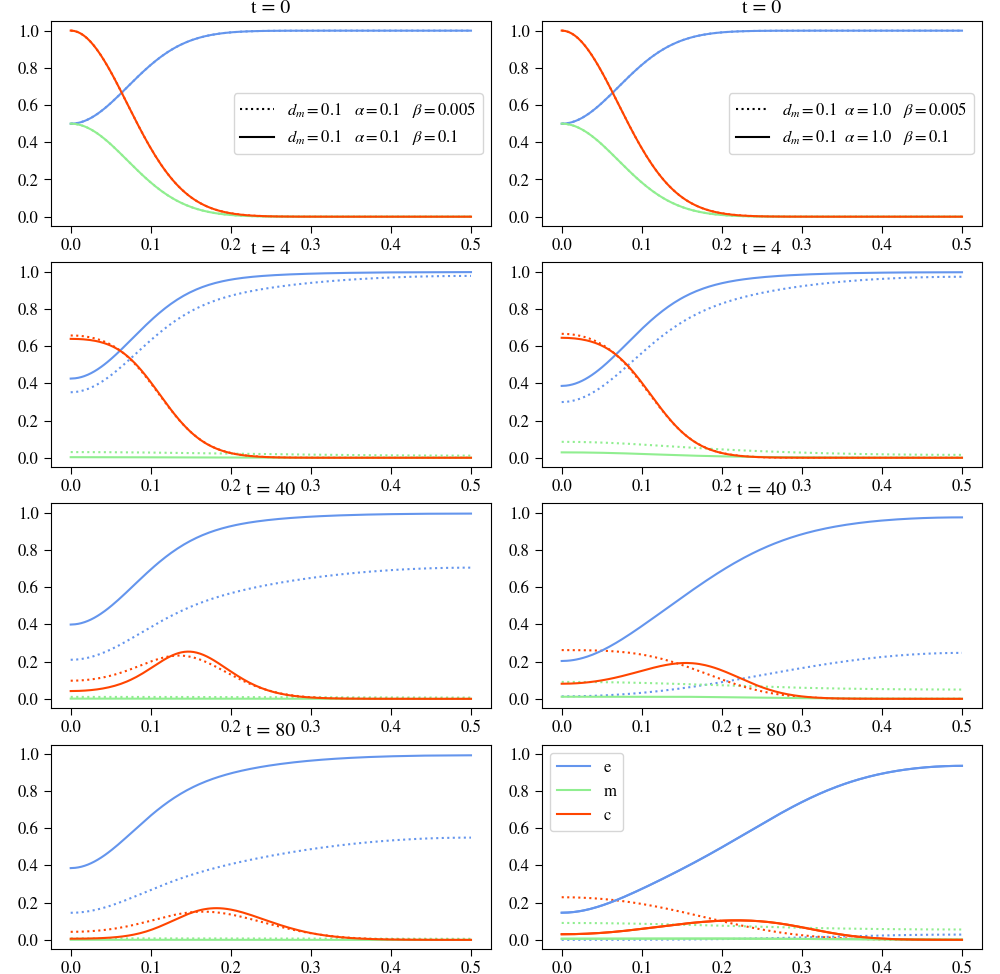
\includegraphics[width=0.85\textwidth]{resources/images/dm_alpha_beta_variation_2.png}
    \caption{Plots show results for varying both $\alpha$ and $\beta$ whilst keeping the other parameters constant, in the images on the left $\alpha=0.1$ with the solid line showing $\beta = 0.005$ and the dotted line $\beta=0.1$ on the right $\alpha=1.0$ with the solid line showing $\beta = 0.005$ and the dotted line $\beta=0.1$.}
    \label{fig:dm_alpha_beta_variation_2}
\end{figure}

Experimenting with all parameters regarding the equation for the matrix-degrading enzymes required to split the results into two figures,~\ref{fig:dm_alpha_beta_variation_1} and ~\ref{fig:dm_alpha_beta_variation_2}, due to clarity reasons. 
We are first going to take a look at the results in figure~\ref{fig:dm_alpha_beta_variation_1}, to see the effect of a decreased diffusion coefficient for the MDEs. We observe that with having $\alpha =0.1$ and $\beta=0.005$ the ECM degradation happens faster due to having a higher MDE concentration, because of lower MDE decay. Which also increases the seperation of the effects of haptotaxis and diffusion on the tumor cells, seperating them into two lumps, one being pulled them along the ECM faster into the tissue the other staying at the origin. Though the MDE concentration diminishes over time we can still see little remaining concentration at the end at $t=8$. Increasing $\beta$ diminishes the MDE concentration sharply, slowing down the ECM degrading process, which increases the effect of haptotaxis over diffusion to pull all of the tumor cells away from the origin to invade the tissue as one lump though at a slower pace. Over time we can see that as expected the tumor cell density's maximum is located approximately right below where $\nabla (c \nabla e)$ is highest. 

Looking at the experiments with higher $\alpha$ values we can see that for lower $\beta$ values the MDE concentration oscilates up and down over time, which indicates that with this configuration of $\alpha$ and $\beta$ values we found a balancing point. For higher $\beta$ values we cannot observe this balance, since in this case the MDEs have nearly decayed after $t=4$. Having such differences in the MDE concentration we can also see big differences in the ECM concentration. Here we see that as expected with $\beta=0.005$ the ECM degradation happens a lot faster than having $\beta=0.1$. These changes in the ECM concentration also affect the tumor cell density. Like in the experiments with $\alpha=0.1$ the results for having higher $\beta$ lead to only one lump invading the tissue with a more even distributed density along the x-axis, whereas lower $\beta$ values made the diffusion and haptotaxis differentiable forming two lumps one to stay at the origin, one to invade the tissue outwards.

Next we are investigating how changing $d_m$ as well will affect the system, looking at figure~\ref{fig:dm_alpha_beta_variation_2}. First of all it is to say that as with varying $d_m$ only the diffusion here is also strong enough to in most cases completely evenly distribute the matrix-degrading enzymes in all of the space after already the fourth step in time. 

On the left side we see the experiments with low $\alpha$ values and see that less decay of the MDEs leads to slower ECM degradataion. Due to the very even distribution of the MDEs we see for both cases a more evenly degradation of the ECM, with overall lower gradients. This results in a longer exposition of haptotatic effects on the tumor cells to form only lump invading the tissue with a moving maximum, though for a lower $\beta$ factor we see that a larger is staying at the origin since the haptotatic pull here is weaker due to having also a more evenly distributed tumor cell density.

Looking at the right side of figure ~\ref{fig:dm_alpha_beta_variation_2} we see with increased $\alpha$ the results regarding the tumor cell density differ strongly. Whereas on the left side we saw that there was always one lump to invade the cells with its maximum moving below where $\nabla(c\nabla e)$ is strongest, we see that for low $\beta$ the lump of tumor cell stays with its core at the origin at $x=0$, where also its maximum is, and invades the tissue with no leading edge. This shows the effect of a both sufficiently fast and efficient degradation of extracellular matrix. Here we see diffusion as the main factor for the movement of the tumor cells since the haptotatic pull is very low, due to small gradients of $e$ only. For the other curves we can observe that as before with rising $\beta$ the ECM degradation pace slows down, in the last point in time the difference $\beta$ causes is pregnantly visible with for low $\beta$ the ECM has been degraded completely but for high $\beta$ there is still a considerable concentration. Looking at the MDE concentration we can also see clear differences regarding the influence of the diffusion on the MDE decay. Though the MDE concentration with high diffusion is more evenly distributed, its overall volume in space is clearly lower than for low diffusion terms, with same $\alpha$ and $\beta$ configuarations.



\subsection{2D Results with Proliferation and Renewal - Homogenous ECM}
In this section we are going to inspect how introducing tumor cell proliferation and extracellular matrix renewal influences the system. Modelled as logistical growth terms, with a limiting factor of spacial occupation, the parameters $\mu_1$ for tumor cell proliferation and $\mu_2$ for extracellular matrix renewal describe their influences. In the previous experiments those parameters were also incorporated, though set to zero. Instead of treating them as parameters to vary, we are inspecting the whole system a new, since they have the potential to drastically change the resulting simulations.

Tumor cell proliferation describes the natural ability of cells to proliferate. Though in the case of the tumor cells the production signalling comes from themselves, surpassing the control chain that limits normal cells to proliferate uncontrollably.

The extracellular matrix is a naturally dynamic structure that undergoes continuous degradation and remodelling. It does this in order to secure tissue development, wound repair tasks, regulate cellular functions or many more tasks. In a model describing the ECM it is crucial to introduce a factor that incorporates these remodelling processes.

As in section~\ref{sec:2D_without_proliferation}, we are using the same inital conditions for all three variables under the assumption we have a homogenous ECM structure. Figure~\ref{fig:2D_homogenous_ECM_initial} depicts these initial conditions on the three variables $c,e,m$ at dimensionless time $t=0$.
\begin{longtable}{|c c c c c c c c c c|}
    \hline
    Figure & Linestyle & $d_c$ & $\gamma$ & $\mu_1$ & $\eta$ & $\mu_2$ & $d_m$ & $\alpha$ & $\beta$ \\ [0.5ex] 
    \hline\hline
    \endfirsthead
    \hline
    Figure & Linestyle & $d_c$ & $\gamma$ & $\mu_1$ & $\eta$ & $\mu_2$ & $d_m$ & $\alpha$ & $\beta$ \\ [0.5ex] 
    \hline\hline
    \endhead
    \hline \multicolumn{10}{|r|}{{continued on next page}} \\ \hline
    \endfoot
    \endlastfoot
    \ref{fig:2D_basecase_comparison} & \sampleline{dotted} & $5\cdot 10^{-4}$ & 0.0055 & 0 & 10 & 0 & $1\cdot 10^{-3}$ & 0.3564 & 0\\ \hline
    \ref{fig:2D_basecase_comparison} & \sampleline{} & $5\cdot 10^{-4}$ & 0.0055 & 0.1 & 10 & 0.5 & $1\cdot 10^{-3}$ & 0.3564 & 0\\ \hline
    \ref{fig:prolif_dc_comparison} & \sampleline{dotted} & $1\cdot 10^{-3}$ & 0.0055 & 0.1 & 10 & 0.5 & $1\cdot 10^{-3}$ & 0.3564 & 0 \\ \hline
    \ref{fig:prolif_dc_comparison} & \sampleline{} & $1\cdot 10^{-4}$ & 0.0055 & 0.1 & 10 & 0.5 & $1\cdot 10^{-3}$ & 0.3564 & 0 \\ \hline 
    \ref{fig:prolif_dc_comparison} & \sampleline{dashed} & $5\cdot 10^{-5}$ & 0.0055 & 0.1 & 10 & 0.5 & $1\cdot 10^{-3}$ & 0.3564 & 0 \\ \hline
    \ref{fig:prolif_gamma_variation} & \sampleline{dotted} & $5\cdot 10^{-4}$ & 0.002 & 0.1 & 10 & 0.5 & $1\cdot 10^{-3}$ & 0.3564 & 0\\  \hline
    \ref{fig:prolif_gamma_variation} & \sampleline{} & $5\cdot 10^{-4}$ & 0.008 & 0.1 & 10 & 0.5 & $1\cdot 10^{-3}$ & 0.3564 & 0\\  \hline
    \ref{fig:prolif_gamma_variation} & \sampleline{dashed} & $5\cdot 10^{-4}$ & 0.01 & 0.1 & 10 & 0.5 & $1\cdot 10^{-3}$ & 0.3564 & 0\\  \hline
    \ref{fig:prolif_mu_1_variation} & \sampleline{dotted} & $5\cdot 10^{-4}$ & 0.0055 & 0 & 10 & 0.5 & $1\cdot 10^{-3}$ & 0.3564 & 0\\  \hline
    \ref{fig:prolif_mu_1_variation} & \sampleline{} & $5\cdot 10^{-4}$ & 0.0055 & 0.5 & 10 & 0.5 & $1\cdot 10^{-3}$ & 0.3564 & 0\\  \hline
    \ref{fig:prolif_mu_1_variation} & \sampleline{dashed} & $5\cdot 10^{-4}$ & 0.0055 & 1.0 & 10 & 0.5 & $1\cdot 10^{-3}$ & 0.3564 & 0\\ \hline
    \ref{fig:prolif_eta_variation} & \sampleline{dotted} & $5\cdot 10^{-4}$ & 0.0055 & 0.1 & 2 & 0.5 & $1\cdot 10^{-3}$ & 0.3564 & 0\\  \hline
    \ref{fig:prolif_eta_variation} & \sampleline{} & $5\cdot 10^{-4}$ & 0.0055 & 0.1 & 12 & 0.5 & $1\cdot 10^{-3}$ & 0.3564 & 0\\  \hline
    \ref{fig:prolif_eta_variation} & \sampleline{dashed} & $5\cdot 10^{-4}$ & 0.0055 & 0.1 & 20 & 0.5 & $1\cdot 10^{-3}$ & 0.3564 & 0\\ \hline
    \ref{fig:prolif_mu_2_variation} & \sampleline{dotted} & $5\cdot 10^{-4}$ & 0.0055 & 0.1 & 10 & 0.1 & $1\cdot 10^{-3}$ & 0.3564 & 0\\ \hline
    \ref{fig:prolif_mu_2_variation} & \sampleline{} & $5\cdot 10^{-4}$ & 0.0055 & 0.1 & 10 & 0.6 & $1\cdot 10^{-3}$ & 0.3564 & 0\\  \hline
    \ref{fig:prolif_mu_2_variation} & \sampleline{dashed} & $5\cdot 10^{-4}$ & 0.0055 & 0.1 & 10 & 1.0 & $1\cdot 10^{-3}$ & 0.3564 & 0\\ \hline
    \ref{fig:prolif_dm_variation} & \sampleline{dotted} & $5\cdot 10^{-4}$ & 0.0055 & 0.1 & 10 & 0.5 & $1\cdot 10^{-3}$ & 0.3564 & 0\\ \hline
    \ref{fig:prolif_dm_variation} & \sampleline{} & $5\cdot 10^{-4}$ & 0.0055 & 0.1 & 10 & 0.5 & $1\cdot 10^{-4}$ & 0.3564 & 0\\  \hline
    \ref{fig:prolif_dm_variation} & \sampleline{dashed} & $5\cdot 10^{-4}$ & 0.0055 & 0.1 & 10 & 0.5 & $1\cdot 10^{-5}$ & 0.3564 & 0\\  \hline
    \ref{fig:prolif_alpha_variation} & \sampleline{dotted} & $5\cdot 10^{-4}$ & 0.0055 & 0.1 & 10 & 0.5 & $1\cdot 10^{-3}$ & 0 & 0 \\ \hline
    \ref{fig:prolif_alpha_variation} & \sampleline{} & $5\cdot 10^{-4}$ & 0.0055 & 0.1 & 10 & 0.5 & $1\cdot 10^{-3}$ & 0.6 & 0 \\ \hline
    \ref{fig:prolif_alpha_variation} & \sampleline{dashed} & $5\cdot 10^{-4}$ & 0.0055 & 0.1 & 10 & 0.5 & $1\cdot 10^{-3}$ & 1.0 & 0 \\ \hline
    \ref{fig:prolif_beta_variation} & \sampleline{dotted} & $5\cdot 10^{-4}$ & 0.0055 & 0.1 & 10 & 0.5 & $1\cdot 10^{-3}$ & 0.3564 & 0.1 \\ \hline
    \ref{fig:prolif_beta_variation} & \sampleline{} & $5\cdot 10^{-4}$ & 0.0055 & 0.1 & 10 & 0.5 & $1\cdot 10^{-3}$ & 0.3564 & 0.01 \\ \hline
    \ref{fig:prolif_beta_variation} & \sampleline{dashed} & $5\cdot 10^{-4}$ & 0.0055 & 0.1 & 10 & 0.5 & $1\cdot 10^{-3}$ & 0.3564 & 0.005 \\ \hline
    \ref{fig:prolif_mu_1_mu_2_variation} - left & \sampleline{dotted} & $5\cdot 10^{-4}$ & 0.0055 & 0.1 & 10 & 0.1 & $1\cdot 10^{-3}$ & 0.3564 & 0 \\ \hline
    \ref{fig:prolif_mu_1_mu_2_variation} - left & \sampleline{} & $5\cdot 10^{-4}$ & 0.0055 & 0.1 & 10 & 1.0 & $1\cdot 10^{-3}$ & 0.3564 & 0 \\ \hline
    \ref{fig:prolif_mu_1_mu_2_variation} - right & \sampleline{dotted} & $5\cdot 10^{-4}$ & 0.0055 & 1.0 & 10 & 0.1 & $1\cdot 10^{-3}$ & 0.3564 & 0 \\ \hline
    \ref{fig:prolif_mu_1_mu_2_variation} - right & \sampleline{} & $5\cdot 10^{-4}$ & 0.0055 & 1.0 & 10 & 1.0 & $1\cdot 10^{-3}$ & 0.3564 & 0 \\ \hline
    \ref{fig:prolif_dc_gamma_mu_1_variation_1} - left & \sampleline{dotted} & $1\cdot 10^{-5}$ & 0.001 & 0.1 & 10 & 0.5 & $1\cdot 10^{-3}$ & 0.3564 & 0 \\ \hline
    \ref{fig:prolif_dc_gamma_mu_1_variation_1} - left & \sampleline{} & $1\cdot 10^{-5}$ & 0.001 & 1.0 & 10 & 0.5 & $1\cdot 10^{-3}$ & 0.3564 & 0 \\ \hline
    \ref{fig:prolif_dc_gamma_mu_1_variation_1} - right & \sampleline{dotted} & $1\cdot 10^{-5}$ & 0.01 & 0.1 & 10 & 0.5 & $1\cdot 10^{-3}$ & 0.3564 & 0 \\ \hline
    \ref{fig:prolif_dc_gamma_mu_1_variation_1} - right & \sampleline{} & $1\cdot 10^{-5}$ & 0.01 & 1.0 & 10 & 0.5 & $1\cdot 10^{-3}$ & 0.3564 & 0 \\ \hline
    \ref{fig:prolif_dc_gamma_mu_1_variation_2} - left & \sampleline{dotted} & $1\cdot 10^{-3}$ & 0.001 & 0.1 & 10 & 0.5 & $1\cdot 10^{-3}$ & 0.3564 & 0 \\ \hline
    \ref{fig:prolif_dc_gamma_mu_1_variation_2} - left & \sampleline{} & $1\cdot 10^{-3}$ & 0.001 & 1.0 & 10 & 0.5 & $1\cdot 10^{-3}$ & 0.3564 & 0 \\ \hline
    \ref{fig:prolif_dc_gamma_mu_1_variation_2} - right & \sampleline{dotted} & $1\cdot 10^{-3}$ & 0.01 & 0.1 & 10 & 0.5 & $1\cdot 10^{-3}$ & 0.3564 & 0 \\ \hline
    \ref{fig:prolif_dc_gamma_mu_1_variation_2} - right & \sampleline{} & $1\cdot 10^{-3}$ & 0.01 & 1.0 & 10 & 0.5 & $1\cdot 10^{-3}$ & 0.3564 & 0 \\ \hline
    \ref{fig:prolif_eta_mu_2_variation} - left & \sampleline{dotted} & $5\cdot 10^{-4}$ & 0.0055 & 0.1 & 2 & 0.1 & $1\cdot 10^{-3}$ & 0.3564 & 0 \\ \hline
    \ref{fig:prolif_eta_mu_2_variation} - left & \sampleline{} & $5\cdot 10^{-4}$ & 0.0055 & 0.1 & 2 & 1.0 & $1\cdot 10^{-3}$ & 0.3564 & 0 \\ \hline
    \ref{fig:prolif_eta_mu_2_variation} - right & \sampleline{dotted} & $5\cdot 10^{-4}$ & 0.0055 & 0.1 & 20 & 0.1 & $1\cdot 10^{-3}$ & 0.3564 & 0 \\ \hline
    \ref{fig:prolif_eta_mu_2_variation} - right & \sampleline{} & $5\cdot 10^{-4}$ & 0.0055 & 0.1 & 20 & 1.0 & $1\cdot 10^{-3}$ & 0.3564 & 0 \\ \hline
    \caption{Overview of all experiments conducted for the model with proliferation and renewal producing 2D output}
    \label{table:2D_experiments_with_proliferation}
\end{longtable}
As in section~\ref{sec:2D_without_proliferation} we see in table~\ref{table:2D_experiments_with_proliferation} a detailed overview of all the experiments done in this section and the parameters used to produce the results. As before do most figures describe multiple experiments, the linestyle of the curve in the figure determines which experiment exactly is described by the set of parameters.


\subsubsection{Basecase Analysis}

\begin{figure}[h]
    \centering
    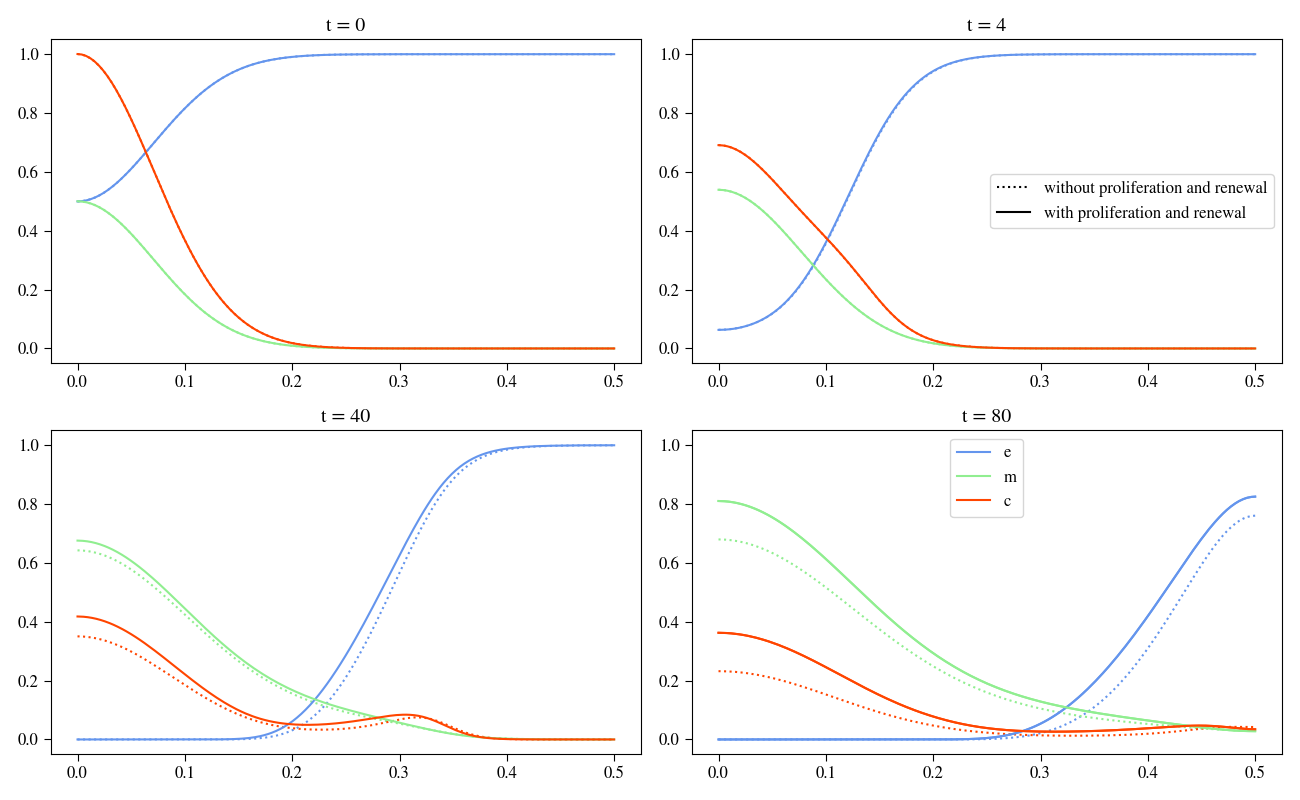
\includegraphics[width=\textwidth]{resources/images/basecase_comparison.png}
    \caption{Describing the updated basecase, in the image above only the updated basecase is plotted, below it is compared to the initial basecase.}
    \label{fig:2D_basecase_comparison}
\end{figure}

It makes sense to establish a basecase to compare the following parameter analysis resulsts against it. In figure~\ref{fig:2D_basecase_comparison} you can see how intoducting tumor cell proliferation and extracellular matrix renewal changes the outcome of the simulation. For this we used the values $\mu_1= 0.1$ and $\mu_2=0.5$ according to the only experiment found for this system of equations in the paper of Kolev et al. \cite{Kolev2010}.

Comparing this new basecase to our initial model's basecase we can see the influences of both $\mu_1$ and $\mu_2$, as for the tumor cell density curve is visibly higher than without proliferation, causing a higher production of matrix-degrading enzymes, which would lead to faster ECM degradation, though this is countered by the renewal factor $\mu_2$ causing the ECM concentration to be higher at the end, at $t=8$, than in the initial basecase experiment.




\subsubsection{Parameter Analysis}

For the Parameter Analysis of the model with proliferation and renewal we are focusing on comparing the results of the updated model with the results produced by the model without renewal and proliferation, this will point out again the influence of $\mu_1$ and $\mu_2$ on the system. 

\subsubsection*{$d_c$ Variation}
\begin{figure}[h]
    \centering
    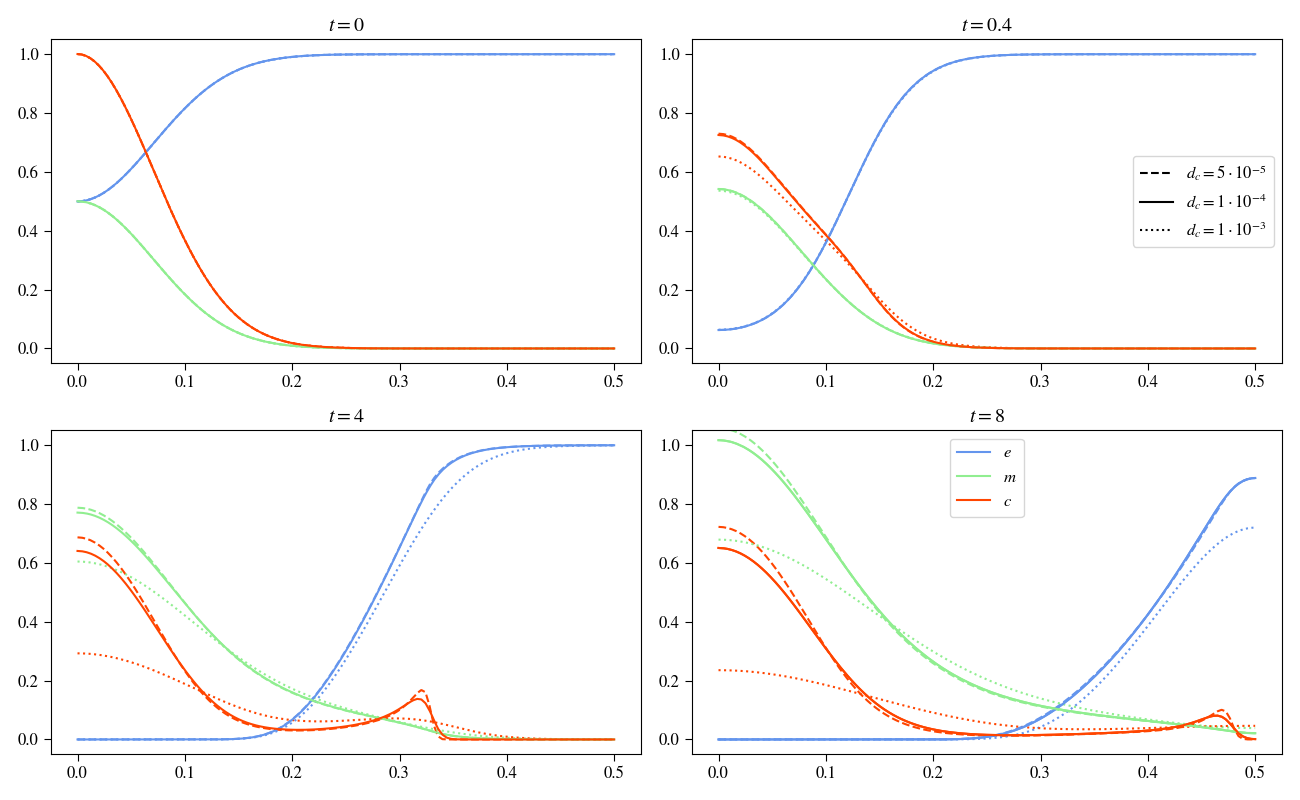
\includegraphics[width=\textwidth]{resources/images/prolif_dc_variation.png}
    \caption{Plots show results for varying $d_c$ whilst keeping the other parameters constant}
    \label{fig:prolif_dc_comparison}
\end{figure}

Varying $d_c$ with proliferation terms, we see the same effects as without proliferation. Higher values for $d_c$ cause a stronger influence of diffusion and a weaker for the haptotaxis, which leads to a curve with less or none of a leading edge invading the space, but to a faster rather constant distribution throughout space. The MDE concentration follows this behaviour, depending on its production on the tumor cell density distribution in space and the ECM is decayed faster, the faster the tissue is invaded, thus the higher the diffusion factor is. Comparing them we see little differences, only tumor cell density and ECM are raised a little in each plot due to the renewal and proliferation factors, which in turn also causes a higher MDE concentration, due to higher tumor cell densities. 


\subsubsection*{$\gamma$ Variation}

\begin{figure}[h]
    \centering
    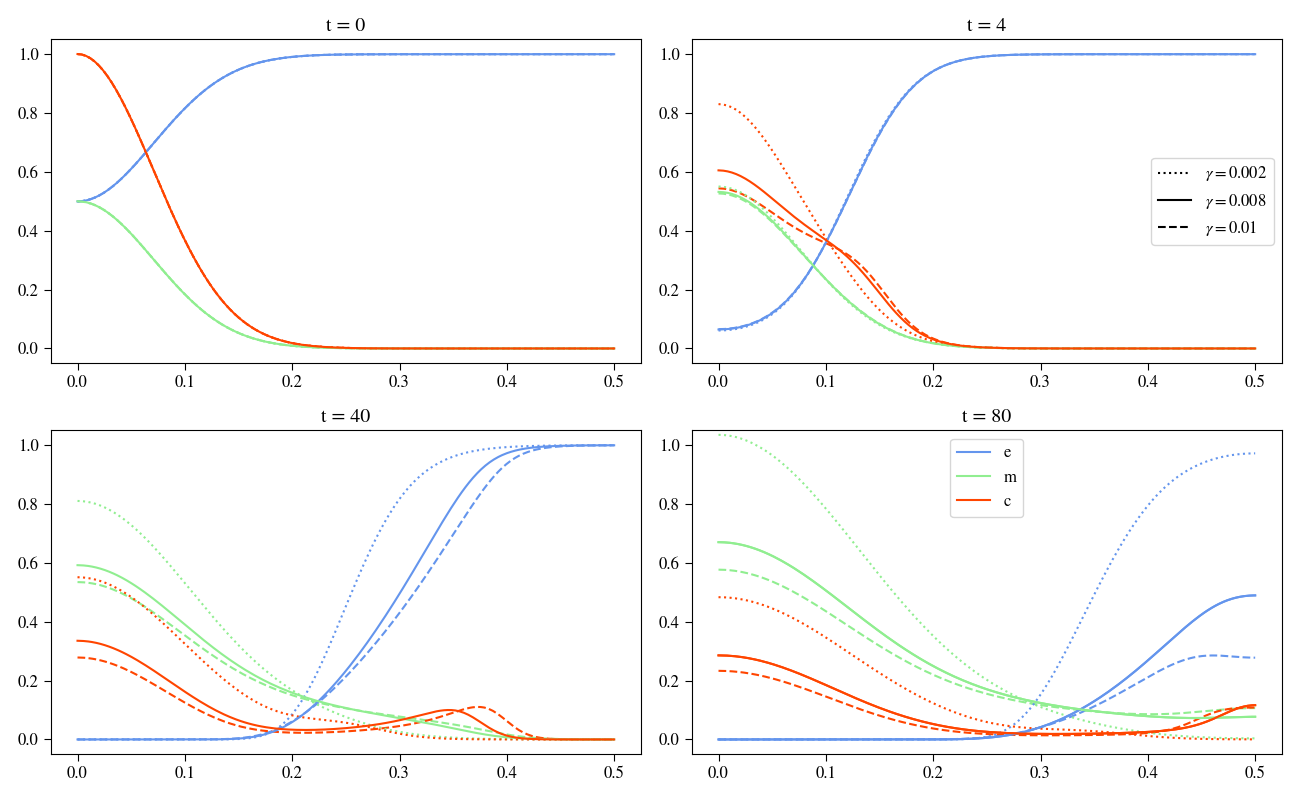
\includegraphics[width=\textwidth]{resources/images/prolif_gamma_variation.png}
    \caption{Plots show results for varying $\gamma$ whilst keeping the other parameters constant.}
    \label{fig:prolif_gamma_variation}
\end{figure}

When we look at $\gamma$ we also can see the same effects as the model without proliferation shows, with the adjustments as varying $d_c$, with raised curves for all variables. Increasing $\gamma$ means increasing haptotaxis effects, pulling the tumor cells stronger towards the extracellular matrix molecules, which causes a faster invasion pace and also a higher density of tumor cells invading the tissue, but a lower staying at the centere at $x=0$. This also means that the ECM degrading process happens faster and the MDEs are more evenly distributed through space the higher $\gamma$ is. As mentioned above the same effects come in this experiment, introducing proliferation and renewal, with higher values for tumor cell density, MDE and ECM concentration especially at the later points in time clearly depictable. It is interessting to observe that though introducing a renewal factor for the extracellular matrix, the proliferation of the tumor cells causes a faster production of matrix-degrading enzymes, which makes the system produce nearly the same results as without proliferation and renewal concerning the ECM concentration, still  it is to say that introducing the renewal of the ECM results in overall slightly higher concentrations of it.

\subsubsection*{$\mu_1$ Variation}
The parameter $\mu_1$ describes the proliferation of the tumor cells, using Kolev et al's estimate in \cite{Kolev2010} we assume an even distribution with $\mu_1 \sim U[0.1, 1.0]$. Introducing this factor we can, wtih an increase of the total amount of tumor cells, expect a faster production of the matrix-degradng enzymes and also a faster degradation of the ECM. Though the effect of the faster ECM degradation might be damped by also introducing a renewal term for it, we can especially for higher $\mu_1$ values expect to dominate the simulations and accellerate ECM degradation.

Since the basecase, using Kolve et al's values, sets the proliferation rate of the tumor cells to $\mu_1=0.1$ we consider in the dotted experiment the effects of only introducing the renewal of the ECM.

\begin{figure}[h]
    \centering
    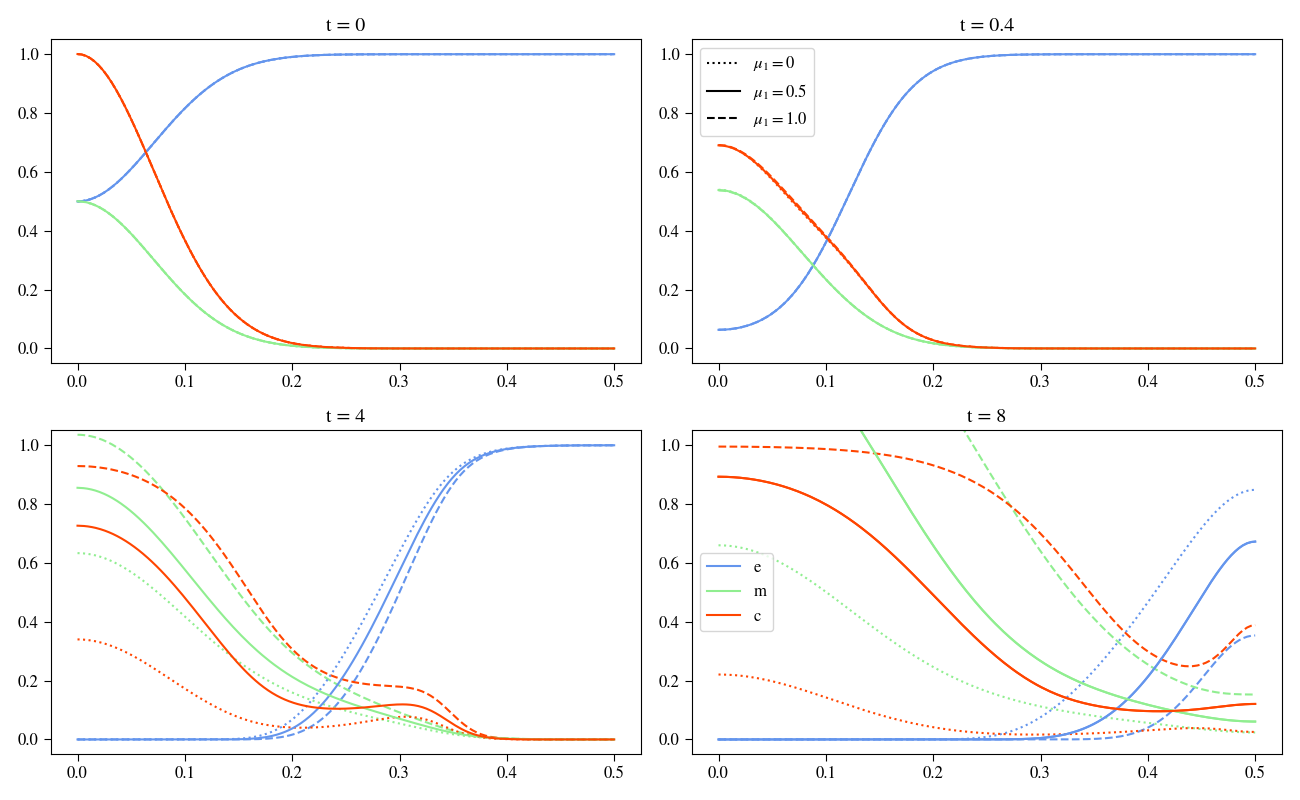
\includegraphics[width=\textwidth]{resources/images/prolif_mu_1_variation.png}
    \caption{Plots show results for varying $\mu_1$ whilst keeping the other parameters constant.}
    \label{fig:prolif_mu_1_variation}
\end{figure}
The effects of $\mu_1$ take some time to act, as we can see no deviations for all the experiments in figure~\ref{fig:prolif_mu_1_variation} at $t=0.4$.

At the next point in time at $t=4$, the differences are striking, concerning all variables. With a higher proliferation factor of the tumor cells, the MDE concentration also rises clearly and the ECM degradation is also accellerated. Yet at this point in time the deviations regarding the curve for the ECM concentration are still subtle.

It looks different in the last point in time at $t=8$. As mentioned above does an increase of total tumor cells drastically increase the MDE concentration and accellerates the ECM degradation.

Introducing $\mu_1$ means introducing one of the hallmarks of cancer; sustaining proliferative signalling, which makes the tumor cells themselves responsible for producing them, instead of requiring other hormones or enzymes to trigger growth signalling. Setting $\mu_1=0$ could be the consequences of a drug working, hindering growth signalling.

\subsubsection*{$\eta$ Variation}
\begin{figure}[h]
    \centering
    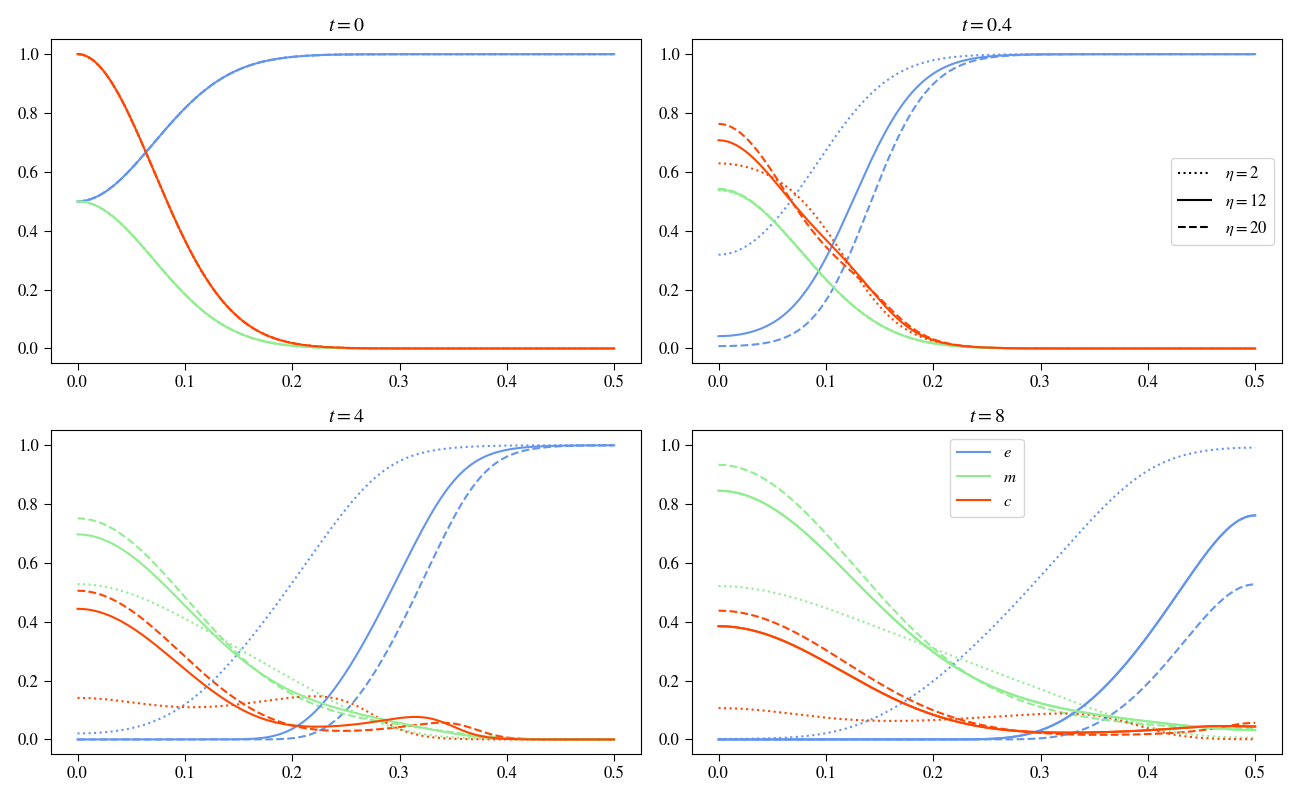
\includegraphics[width=\textwidth]{resources/images/prolif_eta_variation.png}
    \caption{Plots show results for varying $\eta$ whilst keeping the other parameters constant.}
    \label{fig:prolif_eta_variation}
\end{figure}

As we compare the $\eta$ variation between with and without proliferation and renewal models we see mostly the same effects. For the solid and dashed curves we see little though the curves of the new model are all slightly raised. Looking at $\eta=0$ we see some interesting deviations, at the time point $t=0.4$ the plots still look rather similar, but looking at $t=4$ we see that the curve of the tumor cells has a more even distribution along the x-axis and also its maximum is visibly lower with value of about $0.2$ at $x=1.4$ instead of $0.25$ at $x=1.3$. This behaviour is due to the renewal of the ECM, where without proliferation this curve stayed constant throughout the experiment, here it can increase, which it does altering the slope of the curve and therefore influecing the haptotatic pull for the tumor cells, additionally to this the other two experiments showed a visible increase of the tumor cell density and the matrix-degrading enzyme concentration, but only a slight for the ECM concentration, here we can see no increasing of area for the tumor cell density at all. The renewal of the ECM counters the proliferation of the tumor cells and the slowed ECM degrading process in such a way that at the last two point in time we see that the ECM has visibly increased, with both curves ECM and tumor cells almost mirroring each other. Summing up the areas of both variables we see that they toghether occupy the space completely needed for the logistical growth terms, which means that proliferation and renewal will play no more important role continuing with this experiment as they have reached a equlibrium state and cancel each other out. 


\subsubsection*{$\mu_2$ Variation}
The parameter $\mu_2$ describes the renewal processes of the extracellular matrix molecules. Also using Kolev et al's estimate in \cite{Kolev2010} we can assume an even distribution with $\mu_2 \sim U[0.1, 1.0]$. In natural processes the renewal of the extracellular matrix is important to regulate cell differentionation and wound repair for example~\cite{Lu2011-yt}.
\begin{figure}[h]
    \centering
    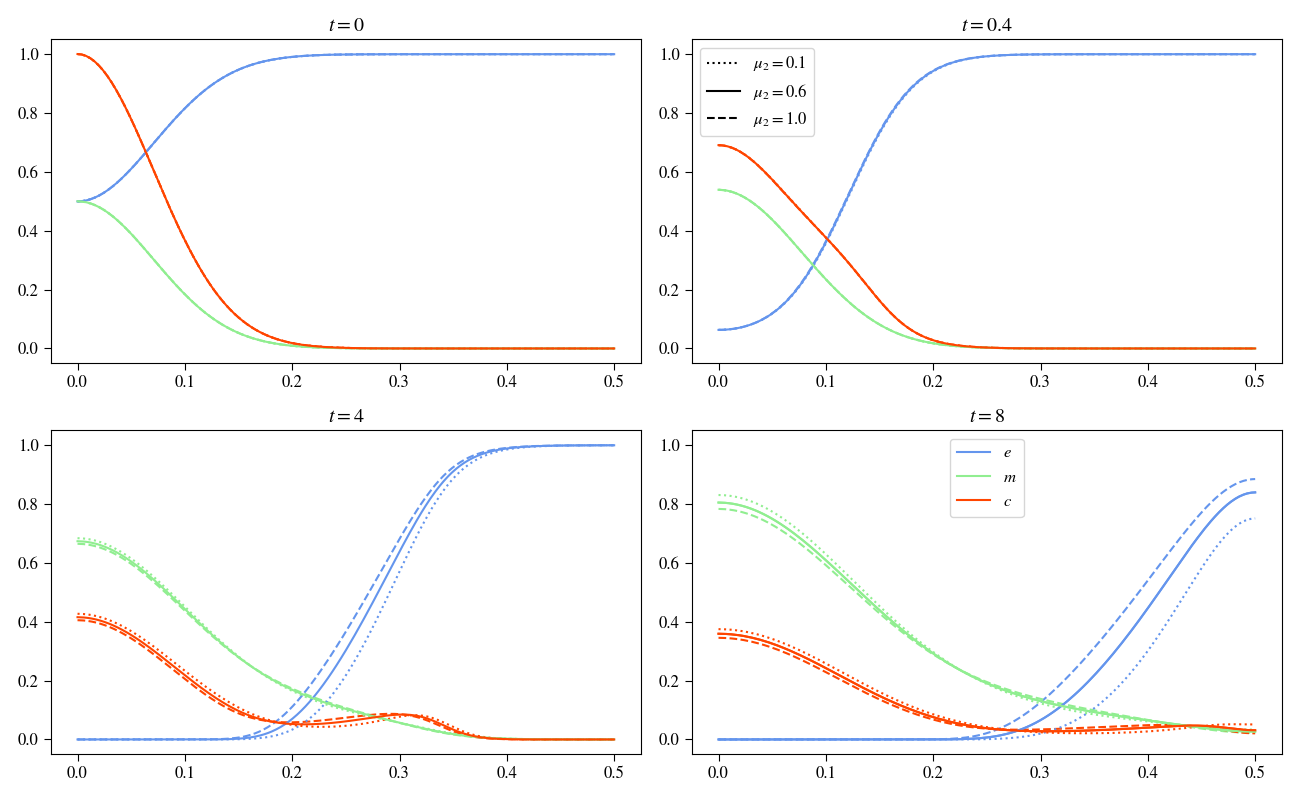
\includegraphics[width=\textwidth]{resources/images/prolif_mu_2_variation.png}
    \caption{Plots show results for varying $\mu_2$ whilst keeping the other parameters constant.}
    \label{fig:prolif_mu_2_variation}
\end{figure}
This renewal process as we see in figure~\ref{fig:prolif_mu_2_variation} takes some time to show effects. There are no deviations for the experiments after $t=0.4$.

Looking at the results later at $t=4$ the differences are still subtle. Increasing $\mu_2$ slows down the extracellular matrix degradation process and with this affects the motility of the tumor cells, pulling less of them outwards into the surrounding tissue. The MDE concentration nearly overlays completely, with a minimal higher concentration for the lowest $\mu_2$ experiment at the origin, due to the also slightly higher tumor cell density at the origin.

The differences at the last point in time at $t=8$ are still minor compared to varying the other parameters. As mentioned before does the slowed ECM degradation diminish haptotatic effects, which leads to slighty less matrix-degrading enzymes concentration at the origin.

We see that varying the ECM renewal rate at this magnitude shows little influence on the resulting simulations.
 
At this point it is important to say that the renewal rates for tissue in the human body strongly vary. Comparing for example bone tissue with connective tissue, we see these processes at highly different time scales. Out of lack of experimental data for this parameter we only investigated Kolev et al's estimates, but considering realistic cases, it is importnatn to have better measures for this parameter.

\subsubsection*{$d_m$ Variation}
\begin{figure}[h!]
    \centering
    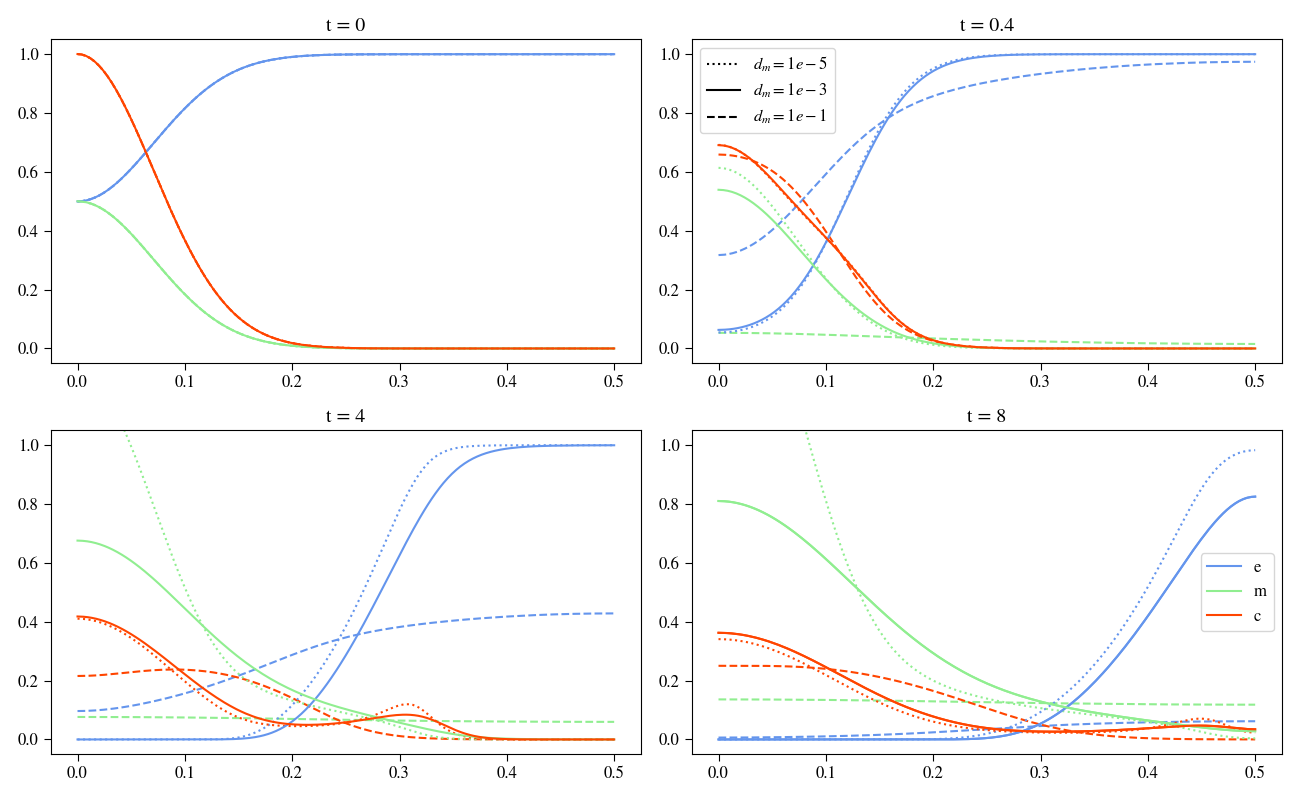
\includegraphics[width=\textwidth]{resources/images/prolif_dm_variation.png}
    \caption{Plots show results for varying $d_m$ whilst keeping the other parameters constant.}
    \label{fig:prolif_dm_variation}
\end{figure}

Comparing the results varying the diffusion factor of the matrix-degrading enzymes does as before yield only minor differences between the initial and updated model. As observed before the tumor cell density's curve and the MDE concentration's curves are slightly raised due to proliferation of the tumor cells. The ECM curve for two lower values of varying $d_m$ though seem to be subject to little to no change, only for very high values of $d_m$ we can see that it is clearly raised comparing it to the model without renewal. The other two curves take off at the some point along the x-axis and finish at the same values for their ECM concentration. Looking at the tumor cell density curves for those $d_m$ values we see that towards $x=0.5$ they don't describe a as steep bump as the initial model. This causes to have little less MDE concentration as well, which is responsible for the seemingly unchanged behaviour of the extracellular matrix concentration.

\subsubsection*{$\alpha$ Variation}
\begin{figure}[h!]
    \centering
    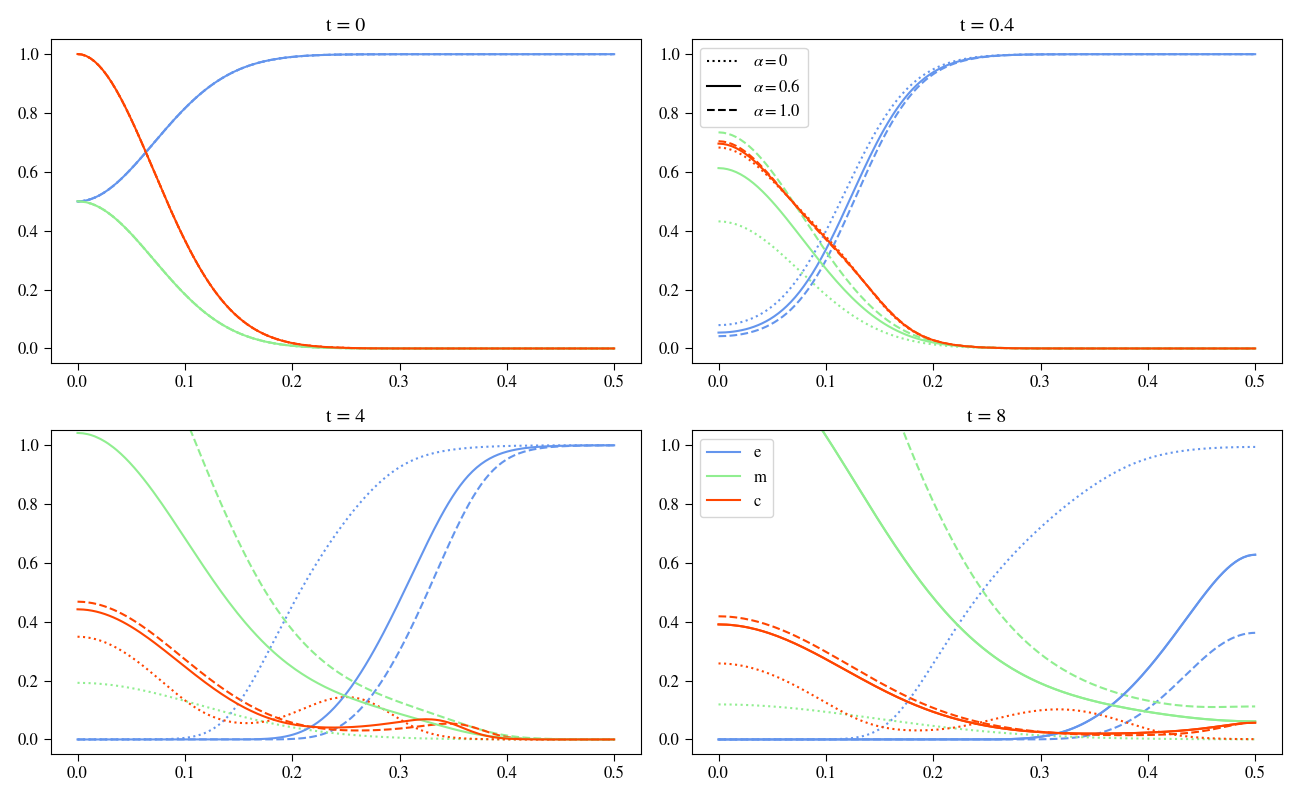
\includegraphics[width=\textwidth]{resources/images/prolif_alpha_variation.png}
    \caption{Plots show results for varying $\alpha$ whilst keeping the other parameters constant.}
    \label{fig:prolif_alpha_variation}
\end{figure}

Taking a look at comparing the $\alpha$-variation yields more interesting results since, $\mu_1$ acts as a secondary MDE production effect by producing tumor cells which in turn produce the matrix-degrading enzymes. We see that though the overall shape and effects to be observed are the same, after $t=4$ the model with proliferation exceeds one at the origin for the MDE concentration for the two higher $\alpha$ experiments, where in the model without proliferation only the one with the highest $\alpha$ value did. The tumor cell denstiy curve is slightly raised, which allows the MDE concentration. Though the higher values for the MDEs leave the ECM degrading process untouched with not clearly visible difference between the inital model and the updated one. 

\subsubsection*{$\beta$ Variation}
\begin{figure}[h!]
    \centering
    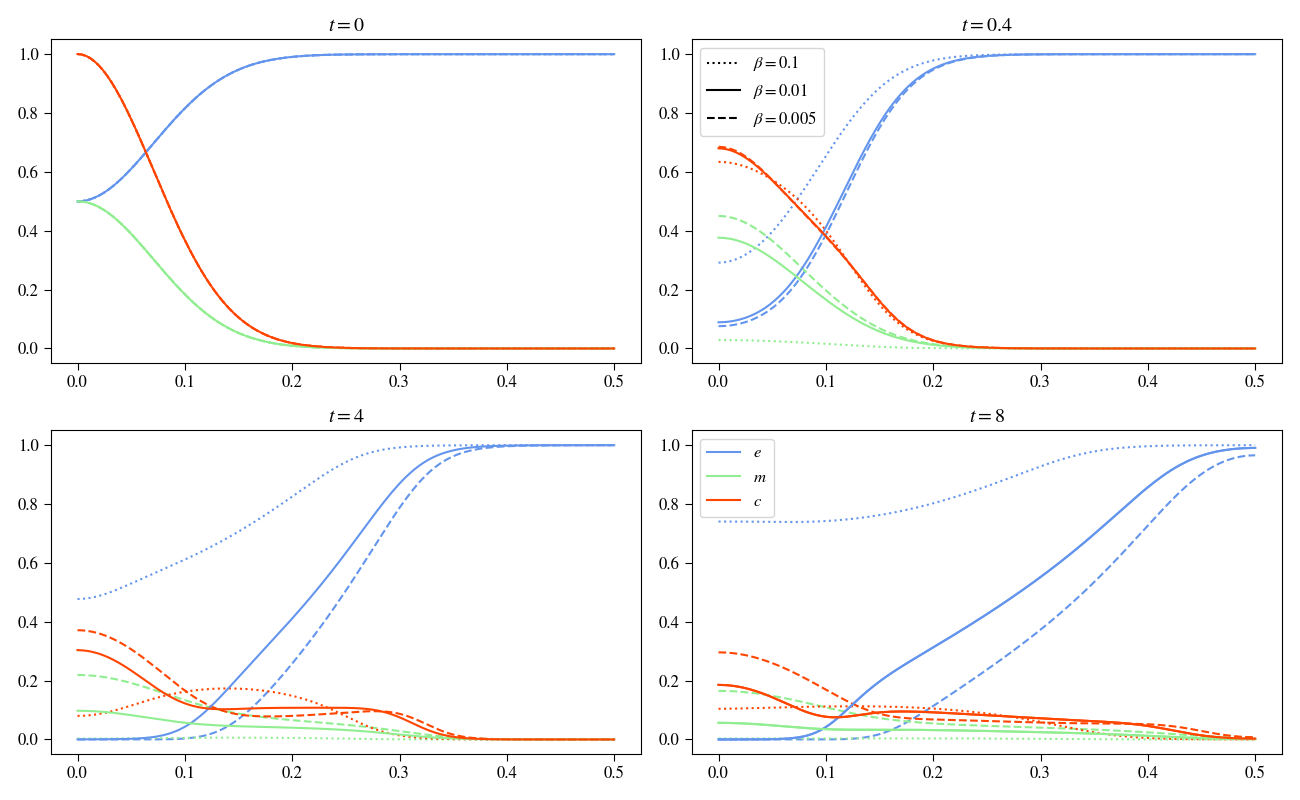
\includegraphics[width=\textwidth]{resources/images/prolif_beta_variation.png}
    \caption{Plots show results for varying $\beta$ whilst keeping the other parameters constant.}
    \label{fig:prolif_beta_variation}
\end{figure}

Considering $\beta$ we can expect that with the introduction of $\mu_2$ the ECM degradation will be slowed considerably with rising $\beta$, since this does not only reduce the MDE concentration but does also renew the ECM. Looking at the plots we can see exactly this behaviour in the dotted line, which shows the experiment results for the highest $\beta$ value of $0.1$. Though even at the end it has an overall area that is slightly less than the inital condition we can see going from timestep $t=0.4$ to $t=4$ that MDE decay and ECM renewal were sufficiently strong to restore the ECM and going from $t=4$ to $t=8$ we see this behaviour again, renewing the ECM. The other two experiments for $\beta$ showed no effects as strong as with $\beta=0.1$, yet we can still see the effects of proliferation and renewal especially clear in the solid line, $\beta=0.01$ at the last point in time, where we can observe a visible increase of both ECM and tumor cell density. In this experiment we see that $\beta$ is a little too low to counter the effects of ECM degradation, going from $t=4$ to $t=8$ we see a clear dicline of ECM concentration though it is not as striking as for $\beta=0.005$. 

\subsubsection*{Cross Variation}

\subsubsection*{$\mu_1 - \mu_2$ Variation}
\begin{figure}[h]
    \centering
    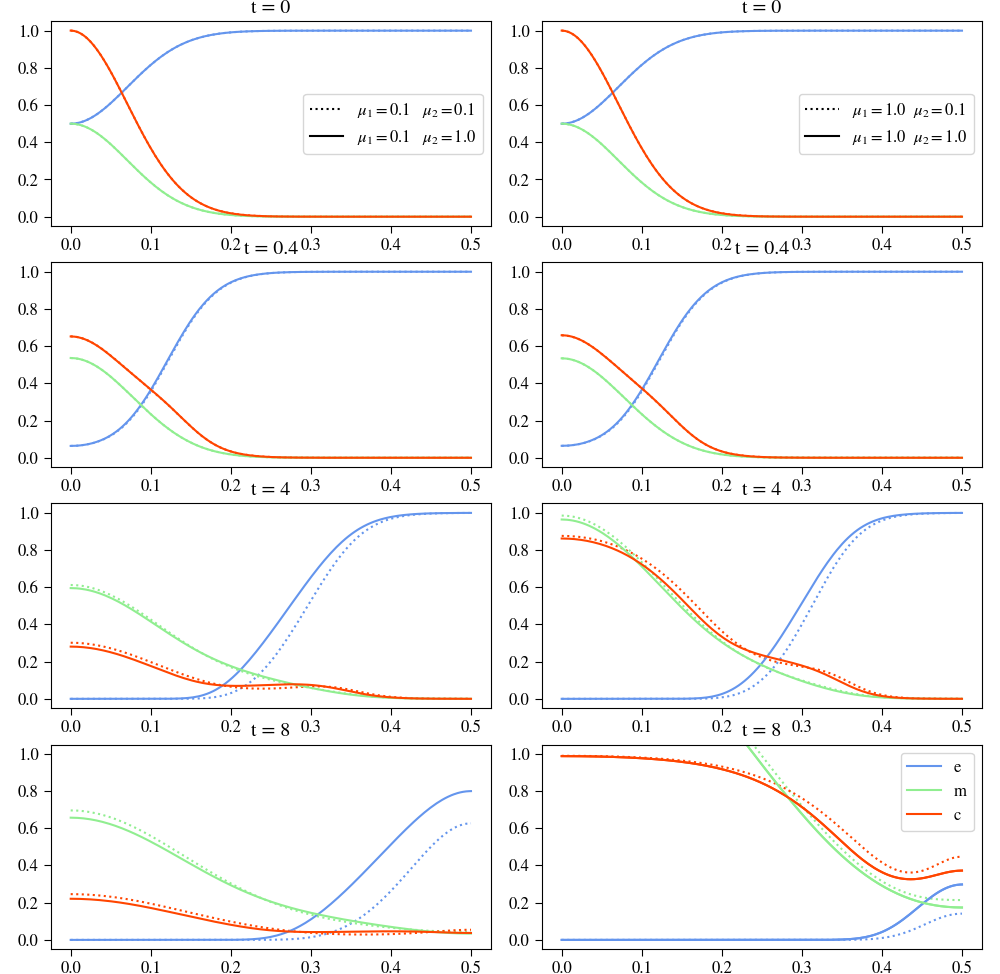
\includegraphics[width=0.85\textwidth]{resources/images/prolif_mu_1_mu_2_variation.png}
    \caption{Plots show results for varying both $\mu_1$ and $\mu_2$ whilst keeping the other parameters constant.}
    \label{fig:prolif_mu_1_mu_2_variation}
\end{figure}
The effects to observe in this cross variation take some time as did the seperate variations of both $\mu_1$ and $\mu_2$. for both $\mu_1=\mu_2=0.1$ we see that slower ECM renewal and slower tumor ell proliferation increase the degrading process of the extracellular matrix and with this affect the haptotaxis effect to increase slightly. At the center a lump remains that has a maximum a little higher than for the experiment with $\mu_2=1.0$ and also the invasion of the tissue has proceeded a little faster. Increasing $\mu_2$, as previously mentioned, results in slower ECM degradation due to the increased renewal term and therefore the tumor cells are stretched out more evenly along the x-axis. Looking at the results when incresing $\mu_1$ we also see the effects only after $t=4$. For $\mu_2=0.1$ we see that the tumor cell density at $x=0$ is slightly larger as well as at $x\approx 2.9$ the curve for $\mu_2=0.1$ is also slightly larger being a little below $\mu_2=1.0$ in between $x\approx 0.2$ and $x\approx 0.29$. The curve for the MDEs looks very similar in both cases for $\mu_2$ due to the very similiar tumor cell density curve, c, though th eECM has visibly faster degraded for $\mu_2=0.1$ due to the slower renewal.

\subsubsection*{$d_c - \gamma - \mu_1$ Variation}
\begin{figure}[h]
    \centering
    \adjustbox{width=0.85\textwidth}{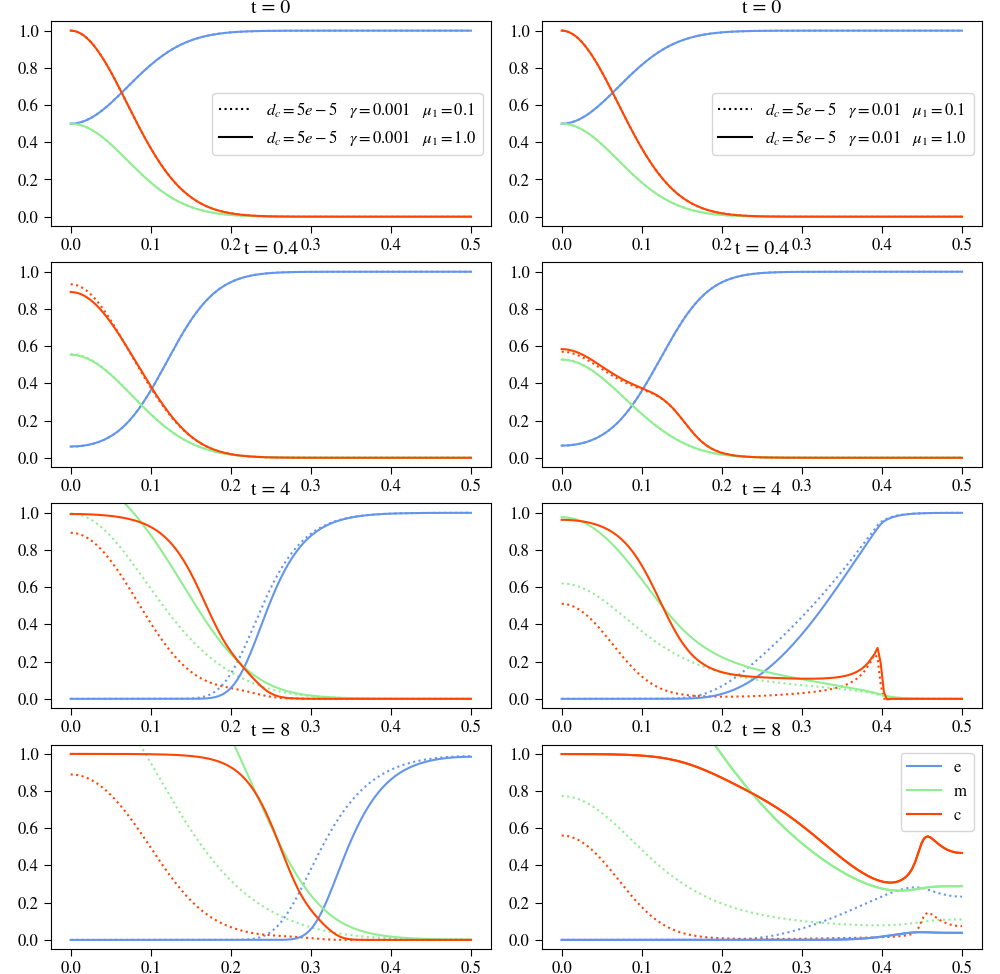
\includegraphics{resources/images/prolif_dc_gamma_mu1_1.png}}
    \caption{Plots show results for varying both $d_c$, $\gamma$ and $\mu_1$ whilst keeping the other parameters constant. This plot is the first of two, with the same $d_c$ value for every plot in this figure.}
    \label{fig:prolif_dc_gamma_mu_1_variation_1}
\end{figure}

\begin{figure}[h]
    \centering
    \adjustbox{width=0.85\textwidth}{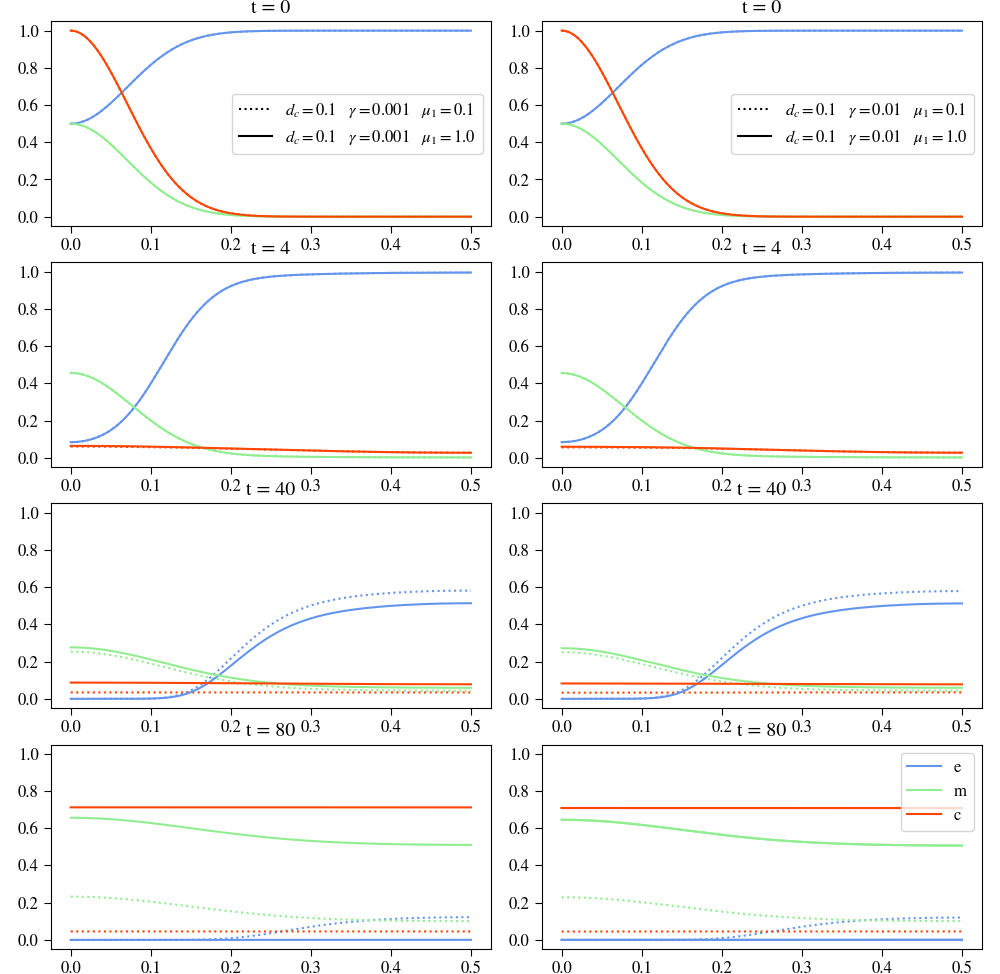
\includegraphics{resources/images/prolif_dc_gamma_mu1_2.png}}
    \caption{Plots show results for varying both $d_c$, $\gamma$ and $\mu_1$ whilst keeping the other parameters constant. This plot is the second of two, with the same $d_c$ value for every plot in this figure.}
    \label{fig:prolif_dc_gamma_mu_1_variation_2}
\end{figure}

First we are goint to take a look at how chaning $\gamma$ and $\mu_1$ affects the system whils having low diffusion values for the tumor cells with $d_c=0.00005$, in figure~\ref{fig:prolif_dc_gamma_mu_1_variation_1}. Inspecting the dotted curve on the left side column, shows the results for all parameters set to low, we see that diffusion is tha mian factor for the movement of the tumor cells, with only little influence of haptotaxis, the tumor cells staying with their maximum at the center. Becasue fo this we also get a high MDE concentration there, but very little excedding the region past $x=0.3$. Due to the MDE also staying centered around thr origin the ECM there is completely degraded, though at $x=0.4$ and further still completely there. Increasing the proliferation factor to $\mu_1=1.0$ shifts the tumor cell density rightwards, making proliferation also a factor for the cell density movement, though keeping the same shape as the low proliferation factor experiment. This right shift causes the MDE concentration to also shift to the right, leading to a faster ECM degradation. Comparing these two experiments already shows the influence of proliferation.

Taking now a look at the right column in figure ~\ref{fig:prolif_dc_gamma_mu_1_variation_1} we see the effects of increased $\gamma$ to $\gamma=1.0$. Foremost we see for the tumor cell density a leading edge developing, seperating it into two lumps, with one staying at the center the other invading the tissue and staying where $\nabla (c \nabla e)$ is highest. With increased $\mu_1$ this secession moving into the tissue is getting more pointy, defying differentiability. After $t=4$ we can observe clear differences regarding ECM and MDE concentration. We see that for higher $\mu_1$ we also get a higher MDE concentration which degrades the ECM visibly faster at the end of the experiments at $t=8$. Though interestingly at $t=4$ the ECM degradataion difference is only minor, at the last point in time the accellerated tumor cell proliferation shows its effet with producignmore MDEs and degrading the ECM considerably faster. What is also interesting to note is that increasing $\gamma$ and keeping $\mu_1$ low the total area of the MDE concentration is lowered also.
Increasing now $d_c$ to $0.1$ we see for all experiments in figure~\ref{fig:prolif_dc_gamma_mu_1_variation_2} that the diffusion of the tumor cells was sufficiently high to evenly distribute the tumor cells constatnly in the space. This constant distribution allows to get an even better look at how $\mu_1$ affects the results, by seeing the lines, describing the tumor cells, rise through time. Looking at the tumor cells over time we can see no observable difference for varying $\gamma$. Haptotaxis effects are completely overlaid by diffusion. We see in the left column that if keeping dc high and $\gamma$ low, but increasing $\mu_1$ leads to higher MDE production rates and also faster ECM degradation. The same behaviour is observable in the right column showing the results for high $\gamma$. That we see no difference is clear, since the tumor cell density development is identical over time as mentioned above. 



\subsubsection*{$\eta -\mu_2$ Variation}
\begin{figure}[h]
    \centering
    \adjustbox{width=0.85\textwidth}{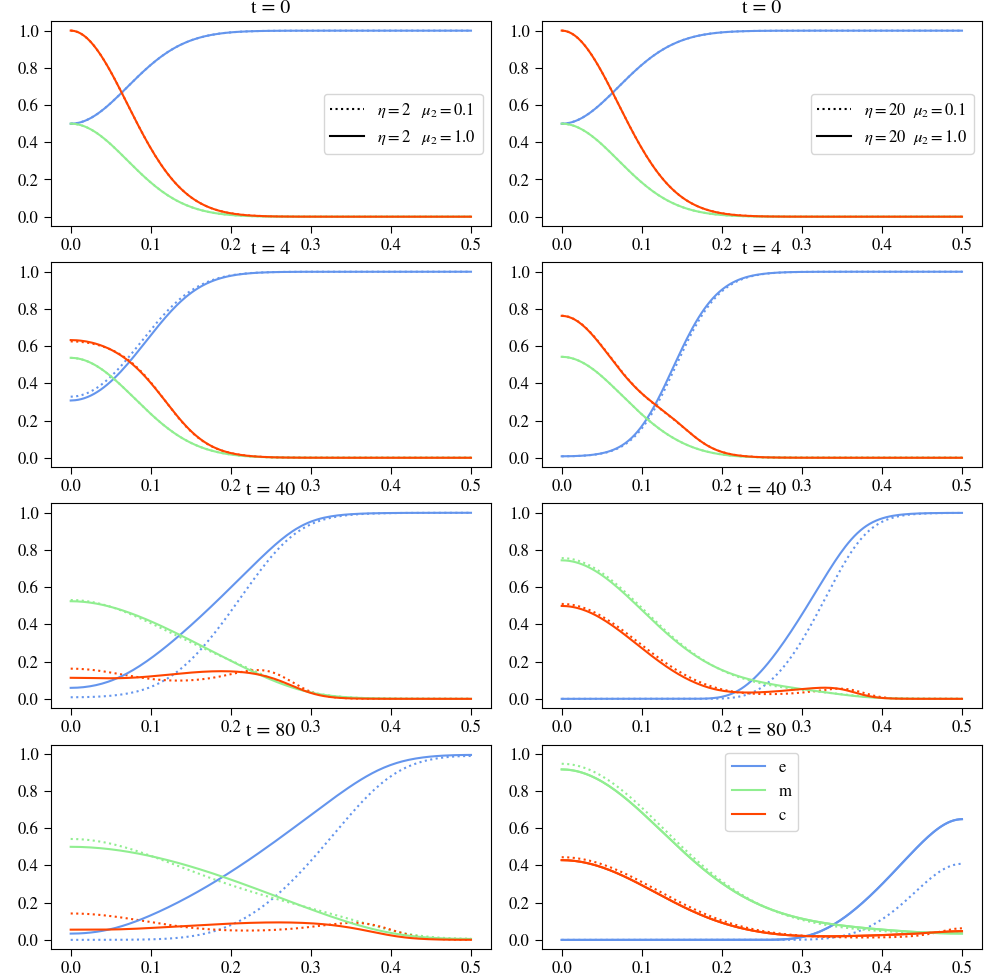
\includegraphics{resources/images/prolif_eta_mu2_variation.png}}
    \caption{Plots show results for varying both $\eta$ and $\mu_2$ whilst keeping the other parameters constant.}
    \label{fig:prolif_eta_mu_2_variation}
\end{figure}

Varying both $\eta$ and $\mu_2$ we can expect to see clear changes in the curve describing the ECM concentration. On the left side of figuer~\ref{fig:prolif_eta_mu_2_variation} we can see the two experiments for low $\eta$ values and see that increasing $\mu_1$ has only a little effect. Where we could have expected to maybe even see an increase of the ECM we see that the ECM curves for both experiments verify that the renewal factor $\mu_2$ was too low to counter the ECM degradation, even with a low degradation factor. Still between $\mu_2=0.1$ and $\mu_2=1.0$ there are visibe differences in the degrading speed of the ECM. We can also observe that with the higher renewal term the tumor cell density curve receives more of an effect of haptotaxis resulting in an more streteched curve with only one long lump of tumor cells, where for the lower renewal factor we can still clearly see that there is a secession that invades the tissue and one that stays at the origin. Concerning the MDE curves we can see little difference, for higher $\mu_2$, which meant more stretched tumor cell density, we can also observe a more stretched MDE curve with a lower maximum at the origin. 

Taking now a look at the experiments with raised $\eta$ to accellerate the ECM degrading process, we can only see pregnant differences in the curve describing the ECM concentration, the other two look across the steps in time to be widely similar. For the ECM curve we see that the experiment with the lower $\mu_2$ value results in a faster degradation process.




\subsection{3D Results with Proliferation and Renewal - Homogenous ECM}
\subsubsection{Basecase Analysis}
\subsubsection{Parameter Analysis}
\lipsum[1-3]




\subsection{2D Results with Proliferation and Renewal - Heterogenous ECM}
\begin{figure}[h]
    \centering
    \label{fig:Initial_Value_Distribution}
    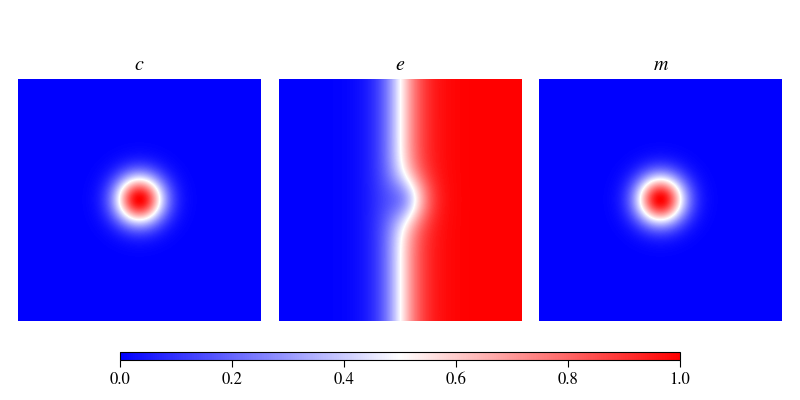
\includegraphics[width=0.85\textwidth]{resources/images/2D_initial_conditions_heterogenous_ECM.png}
    \caption{Visualization of the initial value distribution for an experiment in two space dimensions with a heterogenous extracellular matrix}
    \label{fig:2D_heterogenous_ECM_initial}
\end{figure}
In this section we are investigating how a more realistic structure of the ECM will affect the results of a simulation. We are still using the model with proliferation and renewal. 
For this scenario we assume that there is a nodule of tumor cells already in the center of the simulation that has produced a concentration of matrix-degrading enzymes. Contrary to previous experiments we are assuming that the tumor cells are located at a basement membrane that they already have invaded and are now pushing into the extracellular matrix that lies behind it. These assumptions are described in figure~\ref{fig:tumour_invasion_stage}. We model this in the following experiment with the initial conditions:
\begin{align*}
    c(x,0)= \exp(\frac{-(x-0.5)^2}{0.01})
\end{align*}
\begin{align*}
    m(x,0) = 0.5 c(x,0) = 0.5 \exp(\frac{-(x-0.5)^2}{0.01})
\end{align*}
\begin{align*}
    e(x,0) = 1 - 0.5 c(x,0)
\end{align*}
$\textcolor{red}{insert correct ecm description}$

\begin{figure}[h!]
    \centering
    \adjustbox{width=0.85\textwidth}{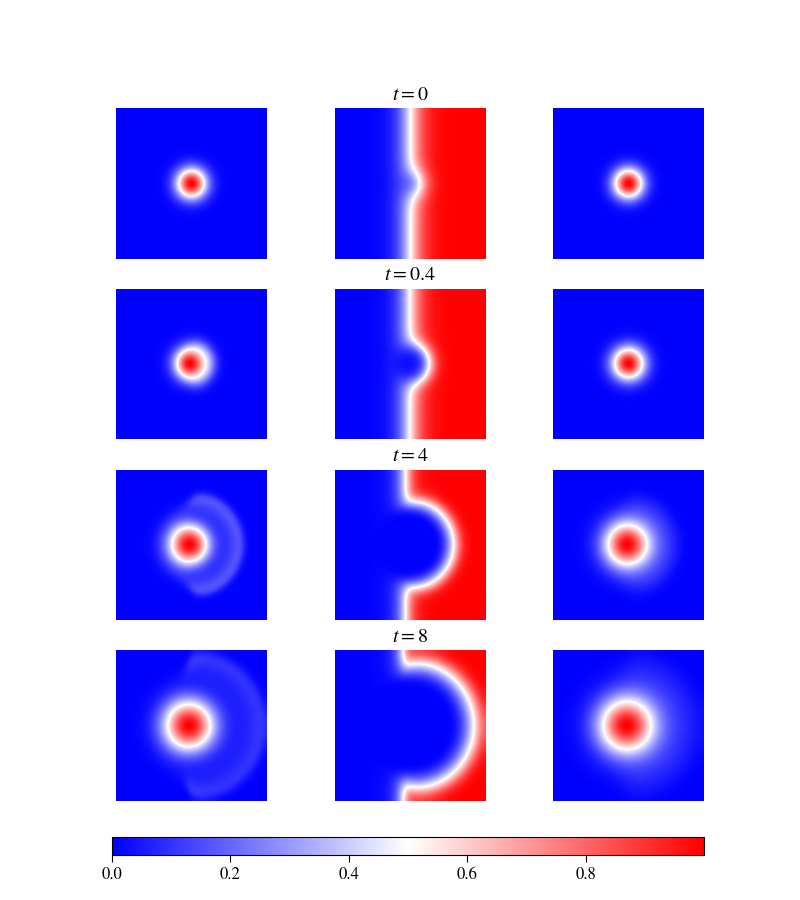
\includegraphics{resources/images/2D_heterogenous_ECM.png}} 
    \caption{2D Results using a heterogenous ECM with the parameter values: $d_c=5\cdot 10^{-4}$, $\gamma=0.0055$, $\mu_1 = 0.1$, $\eta=10$, $\mu_2=0.5$, $d_m = 1\cdot 10^{-3}$, $\alpha = 0.3564$, $\beta = 0$; left: tumor cell density, middle: ECM concentration, right: MDE concentration.}
    \label{fig:2D_heterogenous_ECM}
\end{figure}
Figure~\ref{fig:2D_heterogenous_ECM} you can see the effects using a heterogenous extracellular matrix structure. The plots show in the left column the tumor cell density, the middle column the extracellular matrix concentration and on the right the matrix-degrading enzymes concentration. For the parameters we assumed the basecase studying the model with proliferation. 

This experiment describes a more realistic biological scenarino, like seen in figure~\ref{fig:tumour_invasion_stage}, where the tumor cells are located at the basement membrane of neighboring tissue and have degraded this membrane to invade the surrouding tissue and degrade extracellular matrix there.

In the middle column's first image showing the inital distribution of the experiment you see that the extracellular matrix molecule concentration is only on the right side of the plot, this indicated the neighboring tissue to be invaded. In the center of the same image there is hollow spot where the tumor cells of the initial distribution are located. 

After four timesteps you see that the ECM is slowly being degraded and the tumor cells are being pulled by the ECM concentration further into the neighboring tissue. The concentration of the matrix-degrading enzymes shows little differences comparing their behaviour to the experiments done with a homogenous ECM. They only depend indirectly on the ECM, by being produced where the tumor cells are being pulled by the extracellular matrix concentration. 

The next point in time shows increased ECM degradation with also further invading tumor cells into the tissue. The tumor cells behave as a semicircular wave moving into the direction of the ECM, you can see the main lump remains at the center, with the edge of having containinig a smaller amount of cells moving outwards. The image describing the matrix-degrading enzyme concentration shows still only minor effects, looking closely we can see that from the center moving to the right there is a slightly higher concentration of them than in the other direction.

The last row depicts the experiment after $t=8$ timesteps and we see the aforementioned effects propagated. The ECM degradation has continued as well as the invasion of the tumor cells. The wave moving in direction of the remaining extracellular matrix molecules has spread through space and therefore decreased in its strength. The MDEs still show only little influence of the heterogenous ECM with the main lump staying centered and only difficult to recognize more concentration towards the movement of the tumor cells and concentration of the extracellular matrix.
 
Taking into account different extracellular matrix molecules and structure or physical influences as heat or radiation you can adjust the structure of the ECM and the behaviour of the system to better simulate reallife scenarios of cancer invading tissue.

\subsection{3D Results with Proliferation and Renewal - Heterogenous ECM}